\documentclass[a4paper,14pt,oneside,openany]{memoir}

%%%%%%%%%%%%%%%%%%%%%%%%%%%%%%%%%%%%%%%%%%%%%%%%%%%%%%%%%%%%%%%%%%%%%%%%%%%%%%%%
%%%% Файл упрощённых настроек шаблона, общих для диссертации и автореферата %%%%
%%%%%%%%%%%%%%%%%%%%%%%%%%%%%%%%%%%%%%%%%%%%%%%%%%%%%%%%%%%%%%%%%%%%%%%%%%%%%%%%

%%% Режим черновика %%%
\makeatletter
\@ifundefined{c@draft}{
  \newcounter{draft}
  \setcounter{draft}{0}  % 0 --- чистовик (максимальное соблюдение ГОСТ)
                         % 1 --- черновик (отклонения от ГОСТ, но быстрая
                         %       сборка итоговых PDF)
}{}
\makeatother

%%% Пометки в тексте %%%
\makeatletter
\@ifundefined{c@showmarkup}{
  \newcounter{showmarkup}
  \setcounter{showmarkup}{0}  % 0 --- скрыть пометки
                              % 1 --- показывать пометки
}{}
\makeatother

%%% Использование в pdflatex шрифтов не по-умолчанию %%%
\makeatletter
\@ifundefined{c@usealtfont}{
  \newcounter{usealtfont}
  \setcounter{usealtfont}{1}    % 0 --- шрифты на базе Computer Modern
                                % 1 --- использовать пакет pscyr, при его
                                %       наличии
                                % 2 --- использовать пакет XCharter, при наличии
                                %       подходящей версии
}{}
\makeatother

%%% Использование в xelatex и lualatex семейств шрифтов %%%
\makeatletter
\@ifundefined{c@fontfamily}{
  \newcounter{fontfamily}
  \setcounter{fontfamily}{1}  % 0 --- CMU семейство. Используется как fallback;
                              % 1 --- Шрифты от MS (Times New Roman и компания)
                              % 2 --- Семейство Liberation
}{}
\makeatother


%%% Вывод типов ссылок в библиографии %%%
\makeatletter
\@ifundefined{c@mediadisplay}{
  \newcounter{mediadisplay}
  \setcounter{mediadisplay}{1}   % 0 --- не делать ничего; надписи [Текст] и
                                 %       [Эл. ресурс] будут выводиться только в ссылках с
                                 %       заполненным полем `media`;
                                 % 1 --- автоматически добавлять надпись [Текст] к ссылкам с
                                 %       незаполненным полем `media`; таким образом, у всех
                                 %       источников будет указан тип, что соответствует
                                 %       требованиям ГОСТ
                                 % 2 --- автоматически удалять надписи [Текст], [Эл. Ресурс] и др.;
                                 %       не соответствует ГОСТ
                                 % 3 --- автоматически удалять надпись [Текст];
                                 %       не соответствует ГОСТ
                                 % 4 --- автоматически удалять надпись [Эл. Ресурс];
                                 %       не соответствует ГОСТ
}{}
\makeatother

%%% Предкомпиляция tikz рисунков для ускорения работы %%%
\makeatletter
\@ifundefined{c@imgprecompile}{
  \newcounter{imgprecompile}
  \setcounter{imgprecompile}{0}   % 0 --- без предкомпиляции;
                                  % 1 --- пользоваться предварительно
                                  %       скомпилированными pdf вместо генерации
                                  %       заново из tikz
}{}
\makeatother
            % общие настройки шаблона
%%% Проверка используемого TeX-движка %%%
\newif\ifxetexorluatex   % определяем новый условный оператор (http://tex.stackexchange.com/a/47579)
\ifxetex
    \xetexorluatextrue
\else
    \ifluatex
        \xetexorluatextrue
    \else
        \xetexorluatexfalse
    \fi
\fi

\usepackage{etoolbox}[2015/08/02]   % Для продвинутой проверки разных условий
\providebool{presentation}

\usepackage{comment}    % Позволяет убирать блоки текста (добавляет
                        % окружение comment и команду \excludecomment)

%%% Поля и разметка страницы %%%
\usepackage{pdflscape}  % Для включения альбомных страниц
\usepackage{geometry}   % Для последующего задания полей

%%% Математические пакеты %%%
\usepackage{amsthm,amsmath,amscd}   % Математические дополнения от AMS
\usepackage{amsfonts,amssymb}       % Математические дополнения от AMS
\usepackage{mathtools}              % Добавляет окружение multlined
\usepackage{xfrac}                  % Красивые дроби
\usepackage[
    locale = DE,
    list-separator       = {;\,},
    list-final-separator = {;\,},
    list-pair-separator  = {;\,},
    list-units           = single,
    range-units          = single,
    range-phrase={\text{\ensuremath{-}}},
    % quotient-mode        = fraction, % красивые дроби могут не соответствовать ГОСТ
    fraction-function    = \sfrac,
    separate-uncertainty,
    ]{siunitx}[=v2]                 % Размерности SI
\sisetup{inter-unit-product = \ensuremath{{}\cdot{}}}

% Кириллица в нумерации subequations
% Для правильной работы требуется выполнение сразу после загрузки пакетов
\patchcmd{\subequations}{\def\theequation{\theparentequation\alph{equation}}}
{\def\theequation{\theparentequation\asbuk{equation}}}
{\typeout{subequations patched}}{\typeout{subequations not patched}}

%%%% Установки для размера шрифта 14 pt %%%%
%% Формирование переменных и констант для сравнения (один раз для всех подключаемых файлов)%%
%% должно располагаться до вызова пакета fontspec или polyglossia, потому что они сбивают его работу
\newlength{\curtextsize}
\newlength{\bigtextsize}
\setlength{\bigtextsize}{13.9pt}

\makeatletter
%\show\f@size    % неплохо для отслеживания, но вызывает стопорение процесса,
                 % если документ компилируется без команды  -interaction=nonstopmode
\setlength{\curtextsize}{\f@size pt}
\makeatother

%%% Кодировки и шрифты %%%
\ifxetexorluatex
    \ifpresentation
        \providecommand*\autodot{} % quick fix for polyglossia 1.50
    \fi
    \PassOptionsToPackage{no-math}{fontspec}    % https://tex.stackexchange.com/a/26295/104425
    \usepackage{polyglossia}[2014/05/21]        % Поддержка многоязычности
                                        % (fontspec подгружается автоматически)
\else
   %%% Решение проблемы копирования текста в буфер кракозябрами
    \ifnumequal{\value{usealtfont}}{0}{}{
        \input glyphtounicode.tex
        \input glyphtounicode-cmr.tex %from pdfx package
        \pdfgentounicode=1
    }
    \usepackage{cmap}   % Улучшенный поиск русских слов в полученном pdf-файле
    \ifnumequal{\value{usealtfont}}{2}{}{
        \defaulthyphenchar=127  % Если стоит до fontenc, то переносы
                                % не впишутся в выделяемый текст при
                                % копировании его в буфер обмена
    }
    \usepackage{textcomp}
    \usepackage[T1,T2A]{fontenc}                    % Поддержка русских букв
    \ifnumequal{\value{usealtfont}}{1}{% Используется pscyr, при наличии
        \IfFileExists{pscyr.sty}{\usepackage{pscyr}}{}  % Подключение pscyr
    }{}
    \usepackage[utf8]{inputenc}[2014/04/30]         % Кодировка utf8
    \usepackage[english, russian]{babel}[2014/03/24]% Языки: русский, английский
    \makeatletter\AtBeginDocument{\let\@elt\relax}\makeatother % babel 3.40 fix
    \ifnumequal{\value{usealtfont}}{2}{
        % http://dxdy.ru/post1238763.html#p1238763
        \usepackage[scaled=0.914]{XCharter}[2017/12/19] % Подключение русифицированных шрифтов XCharter
        \usepackage[charter, vvarbb, scaled=1.048]{newtxmath}[2017/12/14]
        \ifpresentation
        \else
            \setDisplayskipStretch{-0.078}
        \fi
    }{}
\fi

%%% Главы, Секции %%%
% \ifpresentation
% \else
%     \usepackage{titlesc}
% \fi

%%% Оформление абзацев %%%
\ifpresentation
\else
    \indentafterchapter     % Красная строка после заголовков типа chapter
    \usepackage{indentfirst}
\fi

%%%
% \usepackage{titlesec} % broken
%%%


%%% Цвета %%%
\ifpresentation
\else
    \usepackage[dvipsnames, table, hyperref]{xcolor} % Совместимо с tikz
\fi

%%% Таблицы %%%
\usepackage{longtable,ltcaption} % Длинные таблицы
\usepackage{multirow,makecell}   % Улучшенное форматирование таблиц
\usepackage{tabu, tabulary}      % таблицы с автоматически подбирающейся
                                 % шириной столбцов (tabu обязательно
                                 % до hyperref вызывать)
\makeatletter
%https://github.com/tabu-issues-for-future-maintainer/tabu/issues/26
\@ifpackagelater{longtable}{2020/02/07}{
\def\tabuendlongtrial{%
    \LT@echunk  \global\setbox\LT@gbox \hbox{\unhbox\LT@gbox}\kern\wd\LT@gbox
                \LT@get@widths
}%
}{}
\makeatother

\usepackage{threeparttable}      % автоматический подгон ширины подписи таблицы

%%% Общее форматирование
\usepackage{soulutf8}% Поддержка переносоустойчивых подчёркиваний и зачёркиваний
\usepackage{icomma}  % Запятая в десятичных дробях

%%% Оптимизация расстановки переносов и длины последней строки абзаца
\IfFileExists{impnattypo.sty}{% проверка установленности пакета impnattypo
    \ifluatex
        \ifnumequal{\value{draft}}{1}{% Черновик
            \usepackage[hyphenation, lastparline, nosingleletter, homeoarchy,
            rivers, draft]{impnattypo}
        }{% Чистовик
            \usepackage[hyphenation, lastparline, nosingleletter]{impnattypo}
        }
    \else
        \usepackage[hyphenation, lastparline]{impnattypo}
    \fi
}{}

%% Векторная графика

\usepackage{tikz}                   % Продвинутый пакет векторной графики
\usetikzlibrary{chains}             % Для примера tikz рисунка
\usetikzlibrary{shapes.geometric}   % Для примера tikz рисунка
\usetikzlibrary{shapes.symbols}     % Для примера tikz рисунка
\usetikzlibrary{arrows}             % Для примера tikz рисунка

%%% Гиперссылки %%%
\ifxetexorluatex
    \let\CYRDZE\relax
\fi
\usepackage{hyperref}[2012/11/06]

%%% Изображения %%%
\usepackage{graphicx}[2014/04/25]   % Подключаем пакет работы с графикой
\usepackage{caption}                % Подписи рисунков и таблиц
\usepackage{subcaption}             % Подписи подрисунков и подтаблиц
\usepackage{pdfpages}               % Добавление внешних pdf файлов
% \usepackage{float}

%%% Счётчики %%%
\usepackage{aliascnt}
\usepackage[figure,table]{totalcount}   % Счётчик рисунков и таблиц (далее \Declare...{lstlisting})
\usepackage{totcount}   % Пакет создания счётчиков на основе последнего номера
                        % подсчитываемого элемента (может требовать дважды
                        % компилировать документ)
\usepackage{totpages}   % Счётчик страниц, совместимый с hyperref (ссылается
                        % на номер последней страницы). Желательно ставить
                        % последним пакетом в преамбуле

%%% Продвинутое управление групповыми ссылками (пока только формулами) %%%
\ifpresentation
\else
    \usepackage[russian]{cleveref} % cleveref имеет сложности со считыванием
    % языка из babel. Такое решение русификации вывода выбрано вместо
    % определения в documentclass из опасности что-то лишнее передать во все
    % остальные пакеты, включая библиографию.

    % Добавление возможности использования пробелов в \labelcref
    % https://tex.stackexchange.com/a/340502/104425
    \usepackage{kvsetkeys}
    \makeatletter
    \let\org@@cref\@cref
    \renewcommand*{\@cref}[2]{%
        \edef\process@me{%
            \noexpand\org@@cref{#1}{\zap@space#2 \@empty}%
        }\process@me
    }
    \makeatother
\fi

\usepackage{placeins} % для \FloatBarrier

\ifnumequal{\value{draft}}{1}{% Черновик
    \usepackage[firstpage]{draftwatermark}
    \SetWatermarkText{DRAFT}
    \SetWatermarkFontSize{14pt}
    \SetWatermarkScale{15}
    \SetWatermarkAngle{45}
}{}

%%% Цитата, не приводимая в автореферате:
% возможно, актуальна только для biblatex
%\newcommand{\citeinsynopsis}[1]{\ifsynopsis\else ~\cite{#1} \fi}

% если текущий процесс запущен библиотекой tikz-external, то прекомпиляция должна быть включена
\ifdefined\tikzexternalrealjob
    \setcounter{imgprecompile}{1}
\fi

\ifnumequal{\value{imgprecompile}}{1}{% Только если у нас включена предкомпиляция
    \usetikzlibrary{external}   % подключение возможности предкомпиляции
    \tikzexternalize[prefix=images/cache/,optimize command away=\includepdf] % activate! % здесь можно указать отдельную папку для скомпилированных файлов
    \ifxetex
        \tikzset{external/up to date check={diff}}
    \fi
}{}




%%% Прикладные пакеты %%%
%\usepackage{calc}               % Пакет для расчётов параметров, например длины

%%% Для добавления Стр. над номерами страниц в оглавлении
%%% http://tex.stackexchange.com/a/306950
\usepackage{afterpage}

%%% Списки %%%
\usepackage{enumitem}

%%% Оформление списка обозначений
\usepackage[intoc]{nomencl}
\makenomenclature
\setlength{\nomitemsep}{-.8\parsep}



\usepackage{fancyhdr}


\usepackage{fr-longtable}    %ради \endlasthead

% Листинги с исходным кодом программ
\usepackage{fancyvrb}
% \usepackage{minted}
\usepackage{listings}
\lccode`\~=0\relax %Без этого хака из-за особенностей пакета listings перестают работать конструкции с \MakeLowercase и т. п. в (xe|lua)latex
\DeclareTotalCounter{lstlisting} % totalcount package

% Русская традиция начертания греческих букв
\usepackage{upgreek} % прямые греческие ради русской традиции

%%% Микротипографика
%\ifnumequal{\value{draft}}{0}{% Только если у нас режим чистовика
	%    \usepackage[final, babel, shrink=45]{microtype}[2016/05/14] % улучшает представление букв и слов в строках, может помочь при наличии отдельно висящих слов
	%}{}

% Отметка о версии черновика на каждой странице
% Чтобы работало надо в своей локальной копии по инструкции
% https://www.ctan.org/pkg/gitinfo2 создать небходимые файлы в папке
% ./git/hooks
% If you’re familiar with tweaking git, you can probably work it out for
% yourself. If not, I suggest you follow these steps:
% 1. First, you need a git repository and working tree. For this example,
% let’s suppose that the root of the working tree is in ~/compsci
% 2. Copy the file post-xxx-sample.txt (which is in the same folder of
% your TEX distribution as this pdf) into the git hooks directory in your
% working copy. In our example case, you should end up with a file called
% ~/compsci/.git/hooks/post-checkout
% 3. If you’re using a unix-like system, don’t forget to make the file executable.
% Just how you do this is outside the scope of this manual, but one
% possible way is with commands such as this:
% chmod g+x post-checkout.
% 4. Test your setup with “git checkout master” (or another suitable branch
% name). This should generate copies of gitHeadInfo.gin in the directories
% you intended.
% 5. Now make two more copies of this file in the same directory (hooks),
% calling them post-commit and post-merge, and you’re done. As before,
% users of unix-like systems should ensure these files are marked as
% executable.
\ifnumequal{\value{draft}}{1}{% Черновик
	\IfFileExists{.git/gitHeadInfo.gin}{
		\usepackage[mark,pcount]{gitinfo2}
		\renewcommand{\gitMark}{rev.\gitAbbrevHash\quad\gitCommitterEmail\quad\gitAuthorIsoDate}
		\renewcommand{\gitMarkFormat}{\rmfamily\color{Gray}\small\bfseries}
	}{}
}{}         % пакеты, которые нужны для шаблона

%%%%%%%%%%%%%%%%%%%%%%%%%%%%%%%%%%%%%%%%%%%%%%%%%%%%%%
%%%% Файл упрощённых настроек шаблона диссертации %%%%
%%%%%%%%%%%%%%%%%%%%%%%%%%%%%%%%%%%%%%%%%%%%%%%%%%%%%%

%%% Инициализирование переменных, не трогать!  %%%
\newcounter{intvl}
\newcounter{otstup}
\newcounter{contnumeq}
\newcounter{contnumfig}
\newcounter{contnumtab}
\newcounter{pgnum}
\newcounter{chapstyle}
\newcounter{headingdelim}
\newcounter{headingalign}
\newcounter{headingsize}
%%%%%%%%%%%%%%%%%%%%%%%%%%%%%%%%%%%%%%%%%%%%%%%%%%%%%%

%%% Область упрощённого управления оформлением %%%

%% Интервал между заголовками и между заголовком и текстом %%
% Заголовки отделяют от текста сверху и снизу
% тремя интервалами (ГОСТ Р 7.0.11-2011, 5.3.5)
\setcounter{intvl}{3}               % Коэффициент кратности к размеру шрифта

%% Отступы у заголовков в тексте %%
\setcounter{otstup}{0}              % 0 --- без отступа; 1 --- абзацный отступ

%% Нумерация формул, таблиц и рисунков %%
% Нумерация формул
\setcounter{contnumeq}{0}   % 0 --- пораздельно (во введении подряд,
                            %       без номера раздела);
                            % 1 --- сквозная нумерация по всей диссертации
% Нумерация рисунков
\setcounter{contnumfig}{1}  % 0 --- пораздельно (во введении подряд,
                            %       без номера раздела);
                            % 1 --- сквозная нумерация по всей диссертации
% Нумерация таблиц
\setcounter{contnumtab}{1}  % 0 --- пораздельно (во введении подряд,
                            %       без номера раздела);
                            % 1 --- сквозная нумерация по всей диссертации

%% Оглавление %%
\setcounter{pgnum}{1}       % 0 --- номера страниц никак не обозначены;
                            % 1 --- Стр. над номерами страниц (дважды
                            %       компилировать после изменения настройки)
\settocdepth{subsection}    % до какого уровня подразделов выносить в оглавление
\setsecnumdepth{subsection} % до какого уровня нумеровать подразделы


%% Текст и форматирование заголовков %%
\setcounter{chapstyle}{1}     % 0 --- разделы только под номером;
                              % 1 --- разделы с названием "Глава" перед номером
\setcounter{headingdelim}{1}  % 0 --- номер отделен пропуском в 1em или \quad;
                              % 1 --- номера разделов и приложений отделены
                              %       точкой с пробелом, подразделы пропуском
                              %       без точки;
                              % 2 --- номера разделов, подразделов и приложений
                              %       отделены точкой с пробелом.

%% Выравнивание заголовков в тексте %%
\setcounter{headingalign}{1}  % 0 --- по центру;
                              % 1 --- по левому краю

%% Размеры заголовков в тексте %%
\setcounter{headingsize}{0}   % 0 --- по ГОСТ, все всегда 14 пт;
                              % 1 --- пропорционально изменяющийся размер
                              %       в зависимости от базового шрифта

%% Подпись таблиц %%

% Смещение строк подписи после первой строки
\newcommand{\tabindent}{0cm}

% Тип форматирования заголовка таблицы:
% plain --- название и текст в одной строке
% split --- название и текст в разных строках
\newcommand{\tabformat}{plain}

%%% Настройки форматирования таблицы `plain`

% Выравнивание по центру подписи, состоящей из одной строки:
% true  --- выравнивать
% false --- не выравнивать
\newcommand{\tabsinglecenter}{false}

% Выравнивание подписи таблиц:
% justified   --- выравнивать как обычный текст («по ширине»)
% centering   --- выравнивать по центру
% centerlast  --- выравнивать по центру только последнюю строку
% centerfirst --- выравнивать по центру только первую строку (не рекомендуется)
% raggedleft  --- выравнивать по правому краю
% raggedright --- выравнивать по левому краю
\newcommand{\tabjust}{justified}

% Разделитель записи «Таблица #» и названия таблицы
\newcommand{\tablabelsep}{~\cyrdash\ }

%%% Настройки форматирования таблицы `split`

% Положение названия таблицы:
% \centering   --- выравнивать по центру
% \raggedleft  --- выравнивать по правому краю
% \raggedright --- выравнивать по левому краю
\newcommand{\splitformatlabel}{\raggedleft}

% Положение текста подписи:
% \centering   --- выравнивать по центру
% \raggedleft  --- выравнивать по правому краю
% \raggedright --- выравнивать по левому краю
\newcommand{\splitformattext}{\raggedright}

%% Подпись рисунков %%
%Разделитель записи «Рисунок #» и названия рисунка
\newcommand{\figlabelsep}{~\cyrdash\ }  % (ГОСТ 2.105, 4.3.1)
                                        % "--- здесь не работает

%%% Цвета гиперссылок %%%
% Latex color definitions: http://latexcolor.com/
\definecolor{linkcolor}{rgb}{0.9,0,0}
\definecolor{citecolor}{rgb}{0,0.6,0}
\definecolor{urlcolor}{rgb}{0,0,1}
%\definecolor{linkcolor}{rgb}{0,0,0} %black
%\definecolor{citecolor}{rgb}{0,0,0} %black
%\definecolor{urlcolor}{rgb}{0,0,0} %black
      % Упрощённые настройки шаблона
\newcommand{\statementOneRU}{
    Ваше первое положение на русском.
}
\newcommand{\statementOneEN}{
    Your first statement in English.
}


\newcommand{\statementTwoRU}{
    Ваше второе положение на русском.
}
\newcommand{\statementTwoEN}{
    Your second statement in English.
} % тут ваши положения 

%%% Кодировки и шрифты %%%
\ifxetexorluatex
    % Язык по-умолчанию русский с поддержкой приятных команд пакета babel
    \setmainlanguage[babelshorthands=true]{russian}
    % Дополнительный язык = английский (в американской вариации по-умолчанию)
    \setotherlanguage{english}

    % Проверка существования шрифтов. Недоступна в pdflatex
    \ifnumequal{\value{fontfamily}}{1}{
        \IfFontExistsTF{Times New Roman}{}{\setcounter{fontfamily}{0}}
    }{}
    \ifnumequal{\value{fontfamily}}{2}{
        \IfFontExistsTF{LiberationSerif}{}{\setcounter{fontfamily}{0}}
    }{}

    \ifnumequal{\value{fontfamily}}{0}{                    % Семейство шрифтов CMU. Используется как fallback
        \setmonofont{CMU Typewriter Text}                  % моноширинный шрифт
        \newfontfamily\cyrillicfonttt{CMU Typewriter Text} % моноширинный шрифт для кириллицы
        \defaultfontfeatures{Ligatures=TeX}                % стандартные лигатуры TeX, замены нескольких дефисов на тире и т. п. Настройки моноширинного шрифта должны идти до этой строки, чтобы при врезках кода программ в коде не применялись лигатуры и замены дефисов
        \setmainfont{CMU Serif}                            % Шрифт с засечками
        \newfontfamily\cyrillicfont{CMU Serif}             % Шрифт с засечками для кириллицы
        \setsansfont{CMU Sans Serif}                       % Шрифт без засечек
        \newfontfamily\cyrillicfontsf{CMU Sans Serif}      % Шрифт без засечек для кириллицы
    }

    \ifnumequal{\value{fontfamily}}{1}{                    % Семейство MS шрифтов
        % \setmonofont{Courier New}                          % моноширинный шрифт
        % \newfontfamily\cyrillicfonttt{Courier New}         % моноширинный шрифт для кириллицы
        \setmonofont{Noto Sans Mono}                          % моноширинный шрифт
        \newfontfamily\cyrillicfonttt{Noto Sans Mono}         % моноширинный шрифт для кириллицы
        \defaultfontfeatures{Ligatures=TeX}                % стандартные лигатуры TeX, замены нескольких дефисов на тире и т. п. Настройки моноширинного шрифта должны идти до этой строки, чтобы при врезках кода программ в коде не применялись лигатуры и замены дефисов
        \setmainfont{Times New Roman}                      % Шрифт с засечками
        \newfontfamily\cyrillicfont{Times New Roman}       % Шрифт с засечками для кириллицы
        \setsansfont{Arial}                                % Шрифт без засечек
        \newfontfamily\cyrillicfontsf{Arial}               % Шрифт без засечек для кириллицы
    }

    \ifnumequal{\value{fontfamily}}{2}{                    % Семейство шрифтов Liberation (https://pagure.io/liberation-fonts)
        \setmonofont{LiberationMono}[Scale=0.87] % моноширинный шрифт
        \newfontfamily\cyrillicfonttt{LiberationMono}[     % моноширинный шрифт для кириллицы
            Scale=0.87]
        \defaultfontfeatures{Ligatures=TeX}                % стандартные лигатуры TeX, замены нескольких дефисов на тире и т. п. Настройки моноширинного шрифта должны идти до этой строки, чтобы при врезках кода программ в коде не применялись лигатуры и замены дефисов
        \setmainfont{LiberationSerif}                      % Шрифт с засечками
        \newfontfamily\cyrillicfont{LiberationSerif}       % Шрифт с засечками для кириллицы
        \setsansfont{LiberationSans}                       % Шрифт без засечек
        \newfontfamily\cyrillicfontsf{LiberationSans}      % Шрифт без засечек для кириллицы
    }

\else
    \ifnumequal{\value{usealtfont}}{1}{% Используется pscyr, при наличии
        \IfFileExists{pscyr.sty}{\renewcommand{\rmdefault}{ftm}}{}
    }{}
\fi

\makeatletter
\newcommand{\verbatimfont}[1]{\def\verbatim@font{#1}}%
\makeatother

\verbatimfont{\normalfont}            % Определение шрифтов (частичное)
%%% Шаблон %%%
\DeclareRobustCommand{\fixme}{\textcolor{red}}  % решаем проблему превращения
                                % названия цвета в результате \MakeUppercase,
                                % http://tex.stackexchange.com/a/187930,
                                % \DeclareRobustCommand protects \fixme
                                % from expanding inside \MakeUppercase
\AtBeginDocument{%
    % \setlength{\parindent}{2.5em}                   % Абзацный отступ. Должен быть одинаковым по всему тексту и равен пяти знакам (ГОСТ Р 7.0.11-2011, 5.3.7).
    \setlength{\parindent}{1.25cm}
}

%%% Таблицы %%%
\DeclareCaptionLabelSeparator{tabsep}{\tablabelsep} % нумерация таблиц
\DeclareCaptionFormat{split}{\splitformatlabel#1\par\splitformattext#3}

\captionsetup[table]{
        format=\tabformat,                % формат подписи (plain|hang)
        font=normal,                      % нормальные размер, цвет, стиль шрифта
        skip=.0pt,                        % отбивка под подписью
        parskip=.0pt,                     % отбивка между параграфами подписи
        position=above,                   % положение подписи
        justification=\tabjust,           % центровка
        indent=\tabindent,                % смещение строк после первой
        labelsep=tabsep,                  % разделитель
        singlelinecheck=\tabsinglecenter, % не выравнивать по центру, если умещается в одну строку
}

%%% Рисунки %%%
\DeclareCaptionLabelSeparator{figsep}{\figlabelsep} % нумерация рисунков

\captionsetup[figure]{
        format=plain,                     % формат подписи (plain|hang)
        font=normal,                      % нормальные размер, цвет, стиль шрифта
        skip=.0pt,                        % отбивка под подписью
        parskip=.0pt,                     % отбивка между параграфами подписи
        position=below,                   % положение подписи
        singlelinecheck=true,             % выравнивание по центру, если умещается в одну строку
        justification=centerlast,         % центровка
        labelsep=figsep,                  % разделитель
}

%%% Подписи подрисунков %%%
\DeclareCaptionSubType{figure}
\renewcommand\thesubfigure{\asbuk{subfigure}} % нумерация подрисунков
\DeclareCaptionFont{norm}{\fontsize{12pt}{16pt}\selectfont}
\newcommand{\subfigureskip}{0.pt}

\captionsetup[subfloat]{
        labelfont=norm,                 % нормальный размер подписей подрисунков
        textfont=norm,                  % нормальный размер подписей подрисунков
        labelsep=space,                 % разделитель
        labelformat=brace,              % одна скобка справа от номера
        justification=centering,        % центровка
        singlelinecheck=true,           % выравнивание по центру, если умещается в одну строку
        skip=\subfigureskip,            % отбивка над подписью
        parskip=.0pt,                   % отбивка между параграфами подписи
        position=below,                 % положение подписи
}

%%% Листинги

% \captionsetup[lstlisting]{format=plain,labelfont=white,textfont=white} 
\captionsetup[lstlisting]{
        format=plain,                     % формат подписи (plain|hang)
        font=rm,                      % нормальные размер, цвет, стиль шрифта
        labelfont=rm,                 % нормальный размер подписей подрисунков
        textfont=rm,                  % нормальный размер подписей подрисунков
        skip=.0pt,                        % отбивка под подписью
        parskip=.0pt,                     % отбивка между параграфами подписи
        position=below,                   % положение подписи
        singlelinecheck=true,             % выравнивание по центру, если умещается в одну строку
        justification=centerlast,         % центровка
        labelsep=figsep,                  % разделитель
}

%%% Настройки ссылок на рисунки, таблицы и др. %%%
% команды \cref...format отвечают за форматирование при помощи команды \cref
% команды \labelcref...format отвечают за форматирование при помощи команды \labelcref

\ifpresentation
\else
    \crefdefaultlabelformat{#2#1#3}

    % Уравнение
    \crefformat{equation}{(#2#1#3)} % одиночная ссылка с приставкой
    \labelcrefformat{equation}{(#2#1#3)} % одиночная ссылка без приставки
    \crefrangeformat{equation}{(#3#1#4) \cyrdash~(#5#2#6)} % диапазон ссылок с приставкой
    \labelcrefrangeformat{equation}{(#3#1#4) \cyrdash~(#5#2#6)} % диапазон ссылок без приставки
    \crefmultiformat{equation}{(#2#1#3)}{ и~(#2#1#3)}{, (#2#1#3)}{ и~(#2#1#3)} % перечисление ссылок с приставкой
    \labelcrefmultiformat{equation}{(#2#1#3)}{ и~(#2#1#3)}{, (#2#1#3)}{ и~(#2#1#3)} % перечисление без приставки

    % Подуравнение
    \crefformat{subequation}{(#2#1#3)} % одиночная ссылка с приставкой
    \labelcrefformat{subequation}{(#2#1#3)} % одиночная ссылка без приставки
    \crefrangeformat{subequation}{(#3#1#4) \cyrdash~(#5#2#6)} % диапазон ссылок с приставкой
    \labelcrefrangeformat{subequation}{(#3#1#4) \cyrdash~(#5#2#6)} % диапазон ссылок без приставки
    \crefmultiformat{subequation}{(#2#1#3)}{ и~(#2#1#3)}{, (#2#1#3)}{ и~(#2#1#3)} % перечисление ссылок с приставкой
    \labelcrefmultiformat{subequation}{(#2#1#3)}{ и~(#2#1#3)}{, (#2#1#3)}{ и~(#2#1#3)} % перечисление без приставки

    % Глава
    \crefformat{chapter}{#2#1#3} % одиночная ссылка с приставкой
    \labelcrefformat{chapter}{#2#1#3} % одиночная ссылка без приставки
    \crefrangeformat{chapter}{#3#1#4 \cyrdash~#5#2#6} % диапазон ссылок с приставкой
    \labelcrefrangeformat{chapter}{#3#1#4 \cyrdash~#5#2#6} % диапазон ссылок без приставки
    \crefmultiformat{chapter}{#2#1#3}{ и~#2#1#3}{, #2#1#3}{ и~#2#1#3} % перечисление ссылок с приставкой
    \labelcrefmultiformat{chapter}{#2#1#3}{ и~#2#1#3}{, #2#1#3}{ и~#2#1#3} % перечисление без приставки

    % Параграф
    \crefformat{section}{#2#1#3} % одиночная ссылка с приставкой
    \labelcrefformat{section}{#2#1#3} % одиночная ссылка без приставки
    \crefrangeformat{section}{#3#1#4 \cyrdash~#5#2#6} % диапазон ссылок с приставкой
    \labelcrefrangeformat{section}{#3#1#4 \cyrdash~#5#2#6} % диапазон ссылок без приставки
    \crefmultiformat{section}{#2#1#3}{ и~#2#1#3}{, #2#1#3}{ и~#2#1#3} % перечисление ссылок с приставкой
    \labelcrefmultiformat{section}{#2#1#3}{ и~#2#1#3}{, #2#1#3}{ и~#2#1#3} % перечисление без приставки

    % Приложение
    \crefformat{appendix}{#2#1#3} % одиночная ссылка с приставкой
    \labelcrefformat{appendix}{#2#1#3} % одиночная ссылка без приставки
    \crefrangeformat{appendix}{#3#1#4 \cyrdash~#5#2#6} % диапазон ссылок с приставкой
    \labelcrefrangeformat{appendix}{#3#1#4 \cyrdash~#5#2#6} % диапазон ссылок без приставки
    \crefmultiformat{appendix}{#2#1#3}{ и~#2#1#3}{, #2#1#3}{ и~#2#1#3} % перечисление ссылок с приставкой
    \labelcrefmultiformat{appendix}{#2#1#3}{ и~#2#1#3}{, #2#1#3}{ и~#2#1#3} % перечисление без приставки

    % Рисунок
    \crefformat{figure}{#2#1#3} % одиночная ссылка с приставкой
    \labelcrefformat{figure}{#2#1#3} % одиночная ссылка без приставки
    \crefrangeformat{figure}{#3#1#4 \cyrdash~#5#2#6} % диапазон ссылок с приставкой
    \labelcrefrangeformat{figure}{#3#1#4 \cyrdash~#5#2#6} % диапазон ссылок без приставки
    \crefmultiformat{figure}{#2#1#3}{ и~#2#1#3}{, #2#1#3}{ и~#2#1#3} % перечисление ссылок с приставкой
    \labelcrefmultiformat{figure}{#2#1#3}{ и~#2#1#3}{, #2#1#3}{ и~#2#1#3} % перечисление без приставки

    % Таблица
    \crefformat{table}{#2#1#3} % одиночная ссылка с приставкой
    \labelcrefformat{table}{#2#1#3} % одиночная ссылка без приставки
    \crefrangeformat{table}{#3#1#4 \cyrdash~#5#2#6} % диапазон ссылок с приставкой
    \labelcrefrangeformat{table}{#3#1#4 \cyrdash~#5#2#6} % диапазон ссылок без приставки
    \crefmultiformat{table}{#2#1#3}{ и~#2#1#3}{, #2#1#3}{ и~#2#1#3} % перечисление ссылок с приставкой
    \labelcrefmultiformat{table}{#2#1#3}{ и~#2#1#3}{, #2#1#3}{ и~#2#1#3} % перечисление без приставки

    % Листинг
    \crefformat{lstlisting}{#2#1#3} % одиночная ссылка с приставкой
    \labelcrefformat{lstlisting}{#2#1#3} % одиночная ссылка без приставки
    \crefrangeformat{lstlisting}{#3#1#4 \cyrdash~#5#2#6} % диапазон ссылок с приставкой
    \labelcrefrangeformat{lstlisting}{#3#1#4 \cyrdash~#5#2#6} % диапазон ссылок без приставки
    \crefmultiformat{lstlisting}{#2#1#3}{ и~#2#1#3}{, #2#1#3}{ и~#2#1#3} % перечисление ссылок с приставкой
    \labelcrefmultiformat{lstlisting}{#2#1#3}{ и~#2#1#3}{, #2#1#3}{ и~#2#1#3} % перечисление без приставки

    % Листинг
    \crefformat{ListingEnv}{#2#1#3} % одиночная ссылка с приставкой
    \labelcrefformat{ListingEnv}{#2#1#3} % одиночная ссылка без приставки
    \crefrangeformat{ListingEnv}{#3#1#4 \cyrdash~#5#2#6} % диапазон ссылок с приставкой
    \labelcrefrangeformat{ListingEnv}{#3#1#4 \cyrdash~#5#2#6} % диапазон ссылок без приставки
    \crefmultiformat{ListingEnv}{#2#1#3}{ и~#2#1#3}{, #2#1#3}{ и~#2#1#3} % перечисление ссылок с приставкой
    \labelcrefmultiformat{ListingEnv}{#2#1#3}{ и~#2#1#3}{, #2#1#3}{ и~#2#1#3} % перечисление без приставки
\fi

%%% Настройки гиперссылок %%%
\ifluatex
    \hypersetup{
        unicode,                % Unicode encoded PDF strings
    }
\fi

\hypersetup{
    linktocpage=true,           % ссылки с номера страницы в оглавлении, списке таблиц и списке рисунков
%    linktoc=all,                % both the section and page part are links
%    pdfpagelabels=false,        % set PDF page labels (true|false)
    plainpages=false,           % Forces page anchors to be named by the Arabic form  of the page number, rather than the formatted form
    colorlinks,                 % ссылки отображаются раскрашенным текстом, а не раскрашенным прямоугольником, вокруг текста
    linkcolor={linkcolor},      % цвет ссылок типа ref, eqref и подобных
    citecolor={citecolor},      % цвет ссылок-цитат
    urlcolor={urlcolor},        % цвет гиперссылок
%    hidelinks,                  % Hide links (removing color and border)
    pdftitle={PhD Thesis},    % Заголовок
    pdfauthor={Author},  % Автор
    pdfsubject={01.04.05 Optics},      % Тема
%    pdfcreator={Создатель},     % Создатель, Приложение
%    pdfproducer={Производитель},% Производитель, Производитель PDF
    pdfkeywords={physics},    % Ключевые слова
    pdflang={ru},
}
\ifnumequal{\value{draft}}{1}{% Черновик
    \hypersetup{
        draft,
    }
}{}


\urlstyle{same}


%%% Списки %%%
% Используем короткое тире (endash) для ненумерованных списков (ГОСТ 2.105-95, пункт 4.1.7, требует дефиса, но так лучше смотрится)
\renewcommand{\labelitemi}{\normalfont\bfseries{--}}

% Перечисление строчными буквами латинского алфавита (ГОСТ 2.105-95, 4.1.7)
%\renewcommand{\theenumi}{\alph{enumi}}
%\renewcommand{\labelenumi}{\theenumi)}

% Перечисление строчными буквами русского алфавита (ГОСТ 2.105-95, 4.1.7)
\makeatletter
\AddEnumerateCounter{\asbuk}{\russian@alph}{щ}      % Управляем списками/перечислениями через пакет enumitem, а он 'не знает' про asbuk, потому 'учим' его
\makeatother
%\renewcommand{\theenumi}{\asbuk{enumi}} %первый уровень нумерации
%\renewcommand{\labelenumi}{\theenumi)} %первый уровень нумерации
\renewcommand{\theenumii}{\asbuk{enumii}} %второй уровень нумерации
\renewcommand{\labelenumii}{\theenumii)} %второй уровень нумерации
\renewcommand{\theenumiii}{\arabic{enumiii}} %третий уровень нумерации
\renewcommand{\labelenumiii}{\theenumiii)} %третий уровень нумерации

\setlist{nosep,%                                    % Единый стиль для всех списков (пакет enumitem), без дополнительных интервалов.
    labelindent=\parindent,leftmargin=*%            % Каждый пункт, подпункт и перечисление записывают с абзацного отступа (ГОСТ 2.105-95, 4.1.8)
}

%%% Правильная нумерация приложений, рисунков и формул %%%
%% По ГОСТ 2.105, п. 4.3.8 Приложения обозначают заглавными буквами русского алфавита,
%% начиная с А, за исключением букв Ё, З, Й, О, Ч, Ь, Ы, Ъ.
%% Здесь также переделаны все нумерации русскими буквами.
\ifxetexorluatex
    \makeatletter
    \def\russian@Alph#1{\ifcase#1\or
       А\or Б\or В\or Г\or Д\or Е\or Ж\or
       И\or К\or Л\or М\or Н\or
       П\or Р\or С\or Т\or У\or Ф\or Х\or
       Ц\or Ш\or Щ\or Э\or Ю\or Я\else\xpg@ill@value{#1}{russian@Alph}\fi}
    \def\russian@alph#1{\ifcase#1\or
       а\or б\or в\or г\or д\or е\or ж\or
       и\or к\or л\or м\or н\or
       п\or р\or с\or т\or у\or ф\or х\or
       ц\or ш\or щ\or э\or ю\or я\else\xpg@ill@value{#1}{russian@alph}\fi}
    \def\cyr@Alph#1{\ifcase#1\or
        А\or Б\or В\or Г\or Д\or Е\or Ж\or
        И\or К\or Л\or М\or Н\or
        П\or Р\or С\or Т\or У\or Ф\or Х\or
        Ц\or Ш\or Щ\or Э\or Ю\or Я\else\xpg@ill@value{#1}{cyr@Alph}\fi}
    \def\cyr@alph#1{\ifcase#1\or
        а\or б\or в\or г\or д\or е\or ж\or
        и\or к\or л\or м\or н\or
        п\or р\or с\or т\or у\or ф\or х\or
        ц\or ш\or щ\or э\or ю\or я\else\xpg@ill@value{#1}{cyr@alph}\fi}
    \makeatother
\else
    \makeatletter
    \if@uni@ode
      \def\russian@Alph#1{\ifcase#1\or
        А\or Б\or В\or Г\or Д\or Е\or Ж\or
        И\or К\or Л\or М\or Н\or
        П\or Р\or С\or Т\or У\or Ф\or Х\or
        Ц\or Ш\or Щ\or Э\or Ю\or Я\else\@ctrerr\fi}
    \else
      \def\russian@Alph#1{\ifcase#1\or
        \CYRA\or\CYRB\or\CYRV\or\CYRG\or\CYRD\or\CYRE\or\CYRZH\or
        \CYRI\or\CYRK\or\CYRL\or\CYRM\or\CYRN\or
        \CYRP\or\CYRR\or\CYRS\or\CYRT\or\CYRU\or\CYRF\or\CYRH\or
        \CYRC\or\CYRSH\or\CYRSHCH\or\CYREREV\or\CYRYU\or
        \CYRYA\else\@ctrerr\fi}
    \fi
    \if@uni@ode
      \def\russian@alph#1{\ifcase#1\or
        а\or б\or в\or г\or д\or е\or ж\or
        и\or к\or л\or м\or н\or
        п\or р\or с\or т\or у\or ф\or х\or
        ц\or ш\or щ\or э\or ю\or я\else\@ctrerr\fi}
    \else
      \def\russian@alph#1{\ifcase#1\or
        \cyra\or\cyrb\or\cyrv\or\cyrg\or\cyrd\or\cyre\or\cyrzh\or
        \cyri\or\cyrk\or\cyrl\or\cyrm\or\cyrn\or
        \cyrp\or\cyrr\or\cyrs\or\cyrt\or\cyru\or\cyrf\or\cyrh\or
        \cyrc\or\cyrsh\or\cyrshch\or\cyrerev\or\cyryu\or
        \cyrya\else\@ctrerr\fi}
    \fi
    \makeatother
\fi


%%http://www.linux.org.ru/forum/general/6993203#comment-6994589 (используется totcount)
\makeatletter
\def\formtotal#1#2#3#4#5{%
    \newcount\@c
    \@c\totvalue{#1}\relax
    \newcount\@last
    \newcount\@pnul
    \@last\@c\relax
    \divide\@last 10
    \@pnul\@last\relax
    \divide\@pnul 10
    \multiply\@pnul-10
    \advance\@pnul\@last
    \multiply\@last-10
    \advance\@last\@c
    #2%
    \ifnum\@pnul=1#5\else%
    \ifcase\@last#5\or#3\or#4\or#4\or#4\else#5\fi
    \fi
}
\makeatother

\newcommand{\formbytotal}[5]{\total{#1}~\formtotal{#1}{#2}{#3}{#4}{#5}}

%%% Команды рецензирования %%%
\ifboolexpr{ (test {\ifnumequal{\value{draft}}{1}}) or (test {\ifnumequal{\value{showmarkup}}{1}})}{
        \newrobustcmd{\todo}[1]{\textcolor{red}{#1}}
        \newrobustcmd{\note}[2][]{\ifstrempty{#1}{#2}{\textcolor{#1}{#2}}}
        \newenvironment{commentbox}[1][]%
        {\ifstrempty{#1}{}{\color{#1}}}%
        {}
}{
        \newrobustcmd{\todo}[1]{}
        \newrobustcmd{\note}[2][]{}
        \excludecomment{commentbox}
}



%%% Переопределение именований, если иначе не сработает %%%
\gappto\captionsrussian{
	   \renewcommand{\chaptername}{ГЛАВА}
	   \renewcommand{\appendixname}{Приложение} % (ГОСТ Р 7.0.11-2011, 5.7)
	}

%%% Изображения %%%
\graphicspath{{images/}{Dissertation/images/}}         % Пути к изображениям

%%% Интервалы %%%
%% По ГОСТ Р 7.0.11-2011, пункту 5.3.6 требуется полуторный интервал
%% Реализация средствами класса (на основе setspace) ближе к типографской классике.
%% И правит сразу и в таблицах (если со звёздочкой)
%\DoubleSpacing*     % Двойной интервал
% \OnehalfSpacing*    % Полуторный интервал
\setSpacing{1.42}   % Полуторный интервал, подобный Ворду (возможно, стоит включать вместе с предыдущей строкой)

%%% Макет страницы %%%
% Выставляем значения полей (ГОСТ 7.0.11-2011, 5.3.7)
% \geometry{a4paper, top=2cm, bottom=2cm, left=3cm, right=1cm, nofoot, nomarginpar, includehead} %, heightrounded, showframe
\geometry{a4paper, top=2cm, bottom=2cm, left=3cm, right=1cm, nofoot, nomarginpar} %, heightrounded, showframe
% \geometry{a4paper, top=2cm, bottom=2cm, left=3cm, right=1cm, nomarginpar} %, heightrounded, showframe
\setlength{\topskip}{0pt}   %размер дополнительного верхнего поля
\setlength{\footskip}{12.3pt} % снимет warning, согласно https://tex.stackexchange.com/a/334346

%%% Выравнивание и переносы %%%
%% http://tex.stackexchange.com/questions/241343/what-is-the-meaning-of-fussy-sloppy-emergencystretch-tolerance-hbadness
%% http://www.latex-community.org/forum/viewtopic.php?p=70342#p70342
\tolerance 1414
\hbadness 1414
\emergencystretch 1.5em % В случае проблем регулировать в первую очередь
\hfuzz 0.3pt
\vfuzz \hfuzz
%\raggedbottom
%\sloppy                 % Избавляемся от переполнений
\clubpenalty=10000      % Запрещаем разрыв страницы после первой строки абзаца
\widowpenalty=10000     % Запрещаем разрыв страницы после последней строки абзаца
\brokenpenalty=4991     % Ограничение на разрыв страницы, если строка заканчивается переносом

%%% Блок управления параметрами для выравнивания заголовков в тексте %%%
\newlength{\otstuplen}
\setlength{\otstuplen}{\theotstup\parindent}
\ifnumequal{\value{headingalign}}{0}{% выравнивание заголовков в тексте
	\newcommand{\hdngalign}{\centering}                % по центру
	\newcommand{\hdngaligni}{}% по центру
	\setlength{\otstuplen}{0pt}
}{%
	\newcommand{\hdngalign}{}                 % по левому краю
	\newcommand{\hdngaligni}{\hspace{\otstuplen}}      % по левому краю
} % В обоих случаях вроде бы без переноса, как и надо (ГОСТ Р 7.0.11-2011, 5.3.5)

%%% Оглавление %%%
\renewcommand{\cftchapterdotsep}{\cftdotsep}                % отбивка точками до номера страницы начала главы/раздела

%% Переносить слова в заголовке не допускается (ГОСТ Р 7.0.11-2011, 5.3.5). Заголовки в оглавлении должны точно повторять заголовки в тексте (ГОСТ Р 7.0.11-2011, 5.2.3). Прямого указания на запрет переносов в оглавлении нет, но по той же логике невнесения искажений в смысл, лучше в оглавлении не переносить:
\setrmarg{2.55em plus1fil}                             %To have the (sectional) titles in the ToC, etc., typeset ragged right with no hyphenation
\renewcommand{\cftchapterpagefont}{\normalfont}        % нежирные номера страниц у глав в оглавлении
\renewcommand{\cftchapterleader}{\cftdotfill{\cftchapterdotsep}}% нежирные точки до номеров страниц у глав в оглавлении
\renewcommand{\cftchapterfont}{\normalfont}                       % нежирные названия глав в оглавлении

\ifnumgreater{\value{headingdelim}}{0}{%
	\renewcommand\cftchapteraftersnum{.\space}       % добавляет точку с пробелом после номера раздела в оглавлении
}{}
\ifnumgreater{\value{headingdelim}}{1}{%
	\renewcommand\cftsectionaftersnum{.\space}       % добавляет точку с пробелом после номера подраздела в оглавлении
	\renewcommand\cftsubsectionaftersnum{.\space}    % добавляет точку с пробелом после номера подподраздела в оглавлении
	\renewcommand\cftsubsubsectionaftersnum{.\space} % добавляет точку с пробелом после номера подподподраздела в оглавлении
	\AfterEndPreamble{% без этого polyglossia сама всё переопределяет
		\setsecnumformat{\csname the#1\endcsname.\space}
	}
}{%
	\AfterEndPreamble{% без этого polyglossia сама всё переопределяет
		\setsecnumformat{\csname the#1\endcsname\quad}
	}
}

\renewcommand*{\cftappendixname}{\appendixname\space} % Слово Приложение в оглавлении

%%% Колонтитулы %%%
% Порядковый номер страницы печатают на середине верхнего поля страницы (ГОСТ Р 7.0.11-2011, 5.3.8)
% \makeevenhead{plain}{}{\rmfamily\thepage}{}
% \makeoddhead{plain}{}{\rmfamily\thepage}{}
% \makeevenfoot{plain}{}{}{}
% \makeoddfoot{plain}{}{}{}
\makeevenhead{plain}{}{}{}
\makeoddhead{plain}{}{}{}
% \makeevenfoot{plain}{}{\rmfamily\thepage}{}
% \makeoddfoot{plain}{}{\rmfamily\thepage}{}
\makeevenfoot{plain}{}{\rmfamily\small\thepage}{}
\makeoddfoot{plain}{}{\rmfamily\small\thepage}{}
\pagestyle{plain}


\fancypagestyle{apppages}{%
\fancyhf{}
\renewcommand{\headrulewidth}{0pt}
\fancyhead[LE,RO]{Продолжение Приложения Б}
}

%%% добавить Стр. над номерами страниц в оглавлении
%%% http://tex.stackexchange.com/a/306950
\newif\ifendTOC

% \newcommand*{\tocheader}{
% 	\ifnumequal{\value{pgnum}}{1}{%
% 		\ifendTOC\else\hbox to \linewidth%
% 		{\noindent{}~\hfill{Стр.}}\par%
% 		\ifnumless{\value{page}}{3}{}{%
% 			\vspace{0.5\onelineskip}
% 		}
% 		\afterpage{\tocheader}
% 		\fi%
% 	}{}%
% }%

%%% Оформление заголовков глав, разделов, подразделов %%%
%% Работа должна быть выполнена ... размером шрифта 12-14 пунктов (ГОСТ Р 7.0.11-2011, 5.3.8). То есть не должно быть надписей шрифтом более 14. Так и поставим.
%% Эти установки будут давать одинаковый результат независимо от выбора базовым шрифтом 12 пт или 14 пт
\newcommand{\basegostsectionfont}{\fontsize{14pt}{16pt}\selectfont\bfseries\normalfont}

\makechapterstyle{thesisgost}{%
	\chapterstyle{default}
	\setlength{\beforechapskip}{0pt}
	\setlength{\midchapskip}{0pt}
	% \setlength{\afterchapskip}{\theintvl\curtextsize}
	\setlength{\afterchapskip}{\baselineskip}
	% \renewcommand*{\chapnamefont}{\basegostsectionfont}
	% \renewcommand*{\chapnumfont}{\basegostsectionfont}
	% \renewcommand*{\chaptitlefont}{\basegostsectionfont}
	\renewcommand*{\chapnamefont}{\normalfont}
	\renewcommand*{\chapnumfont}{\normalfont}
	\renewcommand*{\chaptitlefont}{\normalfont}
	\renewcommand*{\chapterheadstart}{\hspace{\otstuplen}}
	\ifnumgreater{\value{headingdelim}}{0}{%
		\renewcommand*{\afterchapternum}{.\space}   % добавляет точку с пробелом после номера раздела
	}{%
		\renewcommand*{\afterchapternum}{\quad}     % добавляет \quad после номера раздела
	}
	\renewcommand*{\printchapternum}{\hdngalign\chapnumfont \thechapter}
	\renewcommand*{\printchaptername}{}
	\renewcommand*{\printchapternonum}{\hdngalign}
}

\makeatletter
\makechapterstyle{thesisgostchapname}{%
	\chapterstyle{thesisgost}
	\renewcommand*{\printchapternum}{\chapnumfont \thechapter}
	\renewcommand*{\printchaptername}{\hdngalign\chapnamefont \@chapapp} %
}
\makeatother


%%% центрированный

\makechapterstyle{thesisgostcenter}{%
	\chapterstyle{default}
	\setlength{\beforechapskip}{0pt}
	\setlength{\midchapskip}{0pt}
	% \setlength{\afterchapskip}{\theintvl\curtextsize}
	\setlength{\afterchapskip}{\baselineskip}
	% \renewcommand*{\chapnamefont}{\basegostsectionfont}
	% \renewcommand*{\chapnumfont}{\basegostsectionfont}
	% \renewcommand*{\chaptitlefont}{\basegostsectionfont}
	\renewcommand*{\chapnamefont}{\normalfont}
	\renewcommand*{\chapnumfont}{\normalfont}
	\renewcommand*{\chaptitlefont}{\normalfont}
	\renewcommand*{\chapterheadstart}{}
	\ifnumgreater{\value{headingdelim}}{0}{%
		\renewcommand*{\afterchapternum}{.\space}   % добавляет точку с пробелом после номера раздела
	}{%
		\renewcommand*{\afterchapternum}{\quad}     % добавляет \quad после номера раздела
	}
	\renewcommand*{\printchapternum}{\centering\chapnumfont \thechapter}
	\renewcommand*{\printchaptername}{}
	\renewcommand*{\printchapternonum}{\centering}
}

%%%

\makeatletter
\makechapterstyle{thesisgostchapname}{%
	\chapterstyle{thesisgostcenter}
	\renewcommand*{\printchapternum}{\chapnumfont \thechapter}
	\renewcommand*{\printchaptername}{\centering\chapnamefont \@chapapp} %
}
\makeatother


\chapterstyle{thesisgostcenter}

% \setsecheadstyle{\basegostsectionfont\hdngalign}
\setsecheadstyle{\basegostsectionfont\hspace{\otstuplen}}
% \setsecindent{\otstuplen}

% \setsubsecheadstyle{\basegostsectionfont\hdngalign}
\setsubsecheadstyle{\basegostsectionfont\hspace{\otstuplen}}
% \setsubsecindent{\otstuplen}

% \setsubsubsecheadstyle{\basegostsectionfont\hdngalign}
\setsubsubsecheadstyle{\basegostsectionfont\hspace{\otstuplen}}
% \setsubsubsecindent{\otstuplen}

% \sethangfrom{\noindent #1} %все заголовки подразделов центрируются с учетом номера, как block

\ifnumequal{\value{chapstyle}}{1}{%
	\chapterstyle{thesisgostchapname}
	\renewcommand*{\cftchaptername}{\chaptername\space} % будет вписано слово Глава перед каждым номером раздела в оглавлении
}{}%

%%% Интервалы между заголовками
% \setbeforesecskip{\theintvl\curtextsize}% Заголовки отделяют от текста сверху и снизу тремя интервалами (ГОСТ Р 7.0.11-2011, 5.3.5).
% \setaftersecskip{\theintvl\curtextsize}
% \setbeforesubsecskip{\theintvl\curtextsize}
% \setaftersubsecskip{\theintvl\curtextsize}
% \setbeforesubsubsecskip{\theintvl\curtextsize}
% \setaftersubsubsecskip{\theintvl\curtextsize}
\setbeforesecskip{\baselineskip}
\setaftersecskip{\baselineskip}

%%% Вертикальные интервалы глав (\chapter) в оглавлении как и у заголовков
% раскомментировать следующие 2
% \setlength{\cftbeforechapterskip}{0pt plus 0pt}   % ИЛИ эти 2 строки из учебника
% \renewcommand*{\insertchapterspace}{}
% или эту
\renewcommand*{\cftbeforechapterskip}{0em}


%%% Блок дополнительного управления размерами заголовков
\ifnumequal{\value{headingsize}}{1}{% Пропорциональные заголовки и базовый шрифт 14 пт
	% \renewcommand{\basegostsectionfont}{\large\bfseries}
	% \renewcommand*{\chapnamefont}{\Large\bfseries}
	% \renewcommand*{\chapnumfont}{\Large\bfseries}
	% \renewcommand*{\chaptitlefont}{\Large\bfseries}
	\renewcommand{\basegostsectionfont}{\large\bfseries}
	\renewcommand*{\chapnamefont}{\Large\bfseries}
	\renewcommand*{\chapnumfont}{\Large\bfseries}
	\renewcommand*{\chaptitlefont}{\Large\bfseries}
}{}

%%% Счётчики %%%

%% Упрощённые настройки шаблона диссертации: нумерация формул, таблиц, рисунков
\ifnumequal{\value{contnumeq}}{1}{%
	\counterwithout{equation}{chapter} % Убираем связанность номера формулы с номером главы/раздела
}{}
\ifnumequal{\value{contnumfig}}{1}{%
	\counterwithout{figure}{chapter}   % Убираем связанность номера рисунка с номером главы/раздела
}{}
\ifnumequal{\value{contnumtab}}{1}{%
	\counterwithout{table}{chapter}    % Убираем связанность номера таблицы с номером главы/раздела
}{}

\AfterEndPreamble{
	%% регистрируем счётчики в системе totcounter
	\regtotcounter{totalcount@figure}
	\regtotcounter{totalcount@lstlisting}
	\regtotcounter{totalcount@table}       % Если иным способом поставить в преамбуле то ошибка в числе таблиц
	\regtotcounter{TotPages}               % Если иным способом поставить в преамбуле то ошибка в числе страниц
	\newtotcounter{TotPagesNoAppendix} 
	\newtotcounter{totalappendix}
	\newtotcounter{totalchapter}
}


% для вертикального центрирования ячеек в tabulary
\def\zz{\ifx\[$\else\aftergroup\zzz\fi}
%$ \] % <-- чиним подсветку синтаксиса в некоторых редакторах
\def\zzz{\setbox0\lastbox
	\dimen0\dimexpr\extrarowheight + \ht0-\dp0\relax
	\setbox0\hbox{\raise-.5\dimen0\box0}%
	\ht0=\dimexpr\ht0+\extrarowheight\relax
	\dp0=\dimexpr\dp0+\extrarowheight\relax
	\box0
}

% \lstdefinelanguage{Renhanced}%
% {keywords={abbreviate,abline,abs,acos,acosh,action,add1,add,%
% 		aggregate,alias,Alias,alist,all,anova,any,aov,aperm,append,apply,%
% 		approx,approxfun,apropos,Arg,args,array,arrows,as,asin,asinh,%
% 		atan,atan2,atanh,attach,attr,attributes,autoload,autoloader,ave,%
% 		axis,backsolve,barplot,basename,besselI,besselJ,besselK,besselY,%
% 		beta,binomial,body,box,boxplot,break,browser,bug,builtins,bxp,by,%
% 		c,C,call,Call,case,cat,category,cbind,ceiling,character,char,%
% 		charmatch,check,chol,chol2inv,choose,chull,class,close,cm,codes,%
% 		coef,coefficients,co,col,colnames,colors,colours,commandArgs,%
% 		comment,complete,complex,conflicts,Conj,contents,contour,%
% 		contrasts,contr,control,helmert,contrib,convolve,cooks,coords,%
% 		distance,coplot,cor,cos,cosh,count,fields,cov,covratio,wt,CRAN,%
% 		create,crossprod,cummax,cummin,cumprod,cumsum,curve,cut,cycle,D,%
% 		data,dataentry,date,dbeta,dbinom,dcauchy,dchisq,de,debug,%
% 		debugger,Defunct,default,delay,delete,deltat,demo,de,density,%
% 		deparse,dependencies,Deprecated,deriv,description,detach,%
% 		dev2bitmap,dev,cur,deviance,off,prev,,dexp,df,dfbetas,dffits,%
% 		dgamma,dgeom,dget,dhyper,diag,diff,digamma,dim,dimnames,dir,%
% 		dirname,dlnorm,dlogis,dnbinom,dnchisq,dnorm,do,dotplot,double,%
% 		download,dpois,dput,drop,drop1,dsignrank,dt,dummy,dump,dunif,%
% 		duplicated,dweibull,dwilcox,dyn,edit,eff,effects,eigen,else,%
% 		emacs,end,environment,env,erase,eval,equal,evalq,example,exists,%
% 		exit,exp,expand,expression,External,extract,extractAIC,factor,%
% 		fail,family,fft,file,filled,find,fitted,fivenum,fix,floor,for,%
% 		For,formals,format,formatC,formula,Fortran,forwardsolve,frame,%
% 		frequency,ftable,ftable2table,function,gamma,Gamma,gammaCody,%
% 		gaussian,gc,gcinfo,gctorture,get,getenv,geterrmessage,getOption,%
% 		getwd,gl,glm,globalenv,gnome,GNOME,graphics,gray,grep,grey,grid,%
% 		gsub,hasTsp,hat,heat,help,hist,home,hsv,httpclient,I,identify,if,%
% 		ifelse,Im,image,\%in\%,index,influence,measures,inherits,install,%
% 		installed,integer,interaction,interactive,Internal,intersect,%
% 		inverse,invisible,IQR,is,jitter,kappa,kronecker,labels,lapply,%
% 		layout,lbeta,lchoose,lcm,legend,length,levels,lgamma,library,%
% 		licence,license,lines,list,lm,load,local,locator,log,log10,log1p,%
% 		log2,logical,loglin,lower,lowess,ls,lsfit,lsf,ls,machine,Machine,%
% 		mad,mahalanobis,make,link,margin,match,Math,matlines,mat,matplot,%
% 		matpoints,matrix,max,mean,median,memory,menu,merge,methods,min,%
% 		missing,Mod,mode,model,response,mosaicplot,mtext,mvfft,na,nan,%
% 		names,omit,nargs,nchar,ncol,NCOL,new,next,NextMethod,nextn,%
% 		nlevels,nlm,noquote,NotYetImplemented,NotYetUsed,nrow,NROW,null,%
% 		numeric,\%o\%,objects,offset,old,on,Ops,optim,optimise,optimize,%
% 		options,or,order,ordered,outer,package,packages,page,pairlist,%
% 		pairs,palette,panel,par,parent,parse,paste,path,pbeta,pbinom,%
% 		pcauchy,pchisq,pentagamma,persp,pexp,pf,pgamma,pgeom,phyper,pico,%
% 		pictex,piechart,Platform,plnorm,plogis,plot,pmatch,pmax,pmin,%
% 		pnbinom,pnchisq,pnorm,points,poisson,poly,polygon,polyroot,pos,%
% 		postscript,power,ppoints,ppois,predict,preplot,pretty,Primitive,%
% 		print,prmatrix,proc,prod,profile,proj,prompt,prop,provide,%
% 		psignrank,ps,pt,ptukey,punif,pweibull,pwilcox,q,qbeta,qbinom,%
% 		qcauchy,qchisq,qexp,qf,qgamma,qgeom,qhyper,qlnorm,qlogis,qnbinom,%
% 		qnchisq,qnorm,qpois,qqline,qqnorm,qqplot,qr,Q,qty,qy,qsignrank,%
% 		qt,qtukey,quantile,quasi,quit,qunif,quote,qweibull,qwilcox,%
% 		rainbow,range,rank,rbeta,rbind,rbinom,rcauchy,rchisq,Re,read,csv,%
% 		csv2,fwf,readline,socket,real,Recall,rect,reformulate,regexpr,%
% 		relevel,remove,rep,repeat,replace,replications,report,require,%
% 		resid,residuals,restart,return,rev,rexp,rf,rgamma,rgb,rgeom,R,%
% 		rhyper,rle,rlnorm,rlogis,rm,rnbinom,RNGkind,rnorm,round,row,%
% 		rownames,rowsum,rpois,rsignrank,rstandard,rstudent,rt,rug,runif,%
% 		rweibull,rwilcox,sample,sapply,save,scale,scan,scan,screen,sd,se,%
% 		search,searchpaths,segments,seq,sequence,setdiff,setequal,set,%
% 		setwd,show,sign,signif,sin,single,sinh,sink,solve,sort,source,%
% 		spline,splinefun,split,sqrt,stars,start,stat,stem,step,stop,%
% 		storage,strstrheight,stripplot,strsplit,structure,strwidth,sub,%
% 		subset,substitute,substr,substring,sum,summary,sunflowerplot,svd,%
% 		sweep,switch,symbol,symbols,symnum,sys,status,system,t,table,%
% 		tabulate,tan,tanh,tapply,tempfile,terms,terrain,tetragamma,text,%
% 		time,title,topo,trace,traceback,transform,tri,trigamma,trunc,try,%
% 		ts,tsp,typeof,unclass,undebug,undoc,union,unique,uniroot,unix,%
% 		unlink,unlist,unname,untrace,update,upper,url,UseMethod,var,%
% 		variable,vector,Version,vi,warning,warnings,weighted,weights,%
% 		which,while,window,write,\%x\%,x11,X11,xedit,xemacs,xinch,xor,%
% 		xpdrows,xy,xyinch,yinch,zapsmall,zip},%
% 	otherkeywords={!,!=,~,$,*,\%,\&,\%/\%,\%*\%,\%\%,<-,<<-},%$
% 	alsoother={._$},%$
% 	sensitive,%
% 	morecomment=[l]\#,%
% 	morestring=[d]",%
% 	morestring=[d]'% 2001 Robert Denham
% }%

%решаем проблему с кириллицей в комментариях (в pdflatex) https://tex.stackexchange.com/a/103712
\lstset{extendedchars=true,keepspaces=true,literate={Ö}{{\"O}}1
	{Ä}{{\"A}}1
	{Ü}{{\"U}}1
	{ß}{{\ss}}1
	{ü}{{\"u}}1
	{ä}{{\"a}}1
	{ö}{{\"o}}1
	{~}{{\textasciitilde}}1
	{а}{{\selectfont\char224}}1
	{б}{{\selectfont\char225}}1
	{в}{{\selectfont\char226}}1
	{г}{{\selectfont\char227}}1
	{д}{{\selectfont\char228}}1
	{е}{{\selectfont\char229}}1
	{ё}{{\"e}}1
	{ж}{{\selectfont\char230}}1
	{з}{{\selectfont\char231}}1
	{и}{{\selectfont\char232}}1
	{й}{{\selectfont\char233}}1
	{к}{{\selectfont\char234}}1
	{л}{{\selectfont\char235}}1
	{м}{{\selectfont\char236}}1
	{н}{{\selectfont\char237}}1
	{о}{{\selectfont\char238}}1
	{п}{{\selectfont\char239}}1
	{р}{{\selectfont\char240}}1
	{с}{{\selectfont\char241}}1
	{т}{{\selectfont\char242}}1
	{у}{{\selectfont\char243}}1
	{ф}{{\selectfont\char244}}1
	{х}{{\selectfont\char245}}1
	{ц}{{\selectfont\char246}}1
	{ч}{{\selectfont\char247}}1
	{ш}{{\selectfont\char248}}1
	{щ}{{\selectfont\char249}}1
	{ъ}{{\selectfont\char250}}1
	{ы}{{\selectfont\char251}}1
	{ь}{{\selectfont\char252}}1
	{э}{{\selectfont\char253}}1
	{ю}{{\selectfont\char254}}1
	{я}{{\selectfont\char255}}1
	{А}{{\selectfont\char192}}1
	{Б}{{\selectfont\char193}}1
	{В}{{\selectfont\char194}}1
	{Г}{{\selectfont\char195}}1
	{Д}{{\selectfont\char196}}1
	{Е}{{\selectfont\char197}}1
	{Ё}{{\"E}}1
	{Ж}{{\selectfont\char198}}1
	{З}{{\selectfont\char199}}1
	{И}{{\selectfont\char200}}1
	{Й}{{\selectfont\char201}}1
	{К}{{\selectfont\char202}}1
	{Л}{{\selectfont\char203}}1
	{М}{{\selectfont\char204}}1
	{Н}{{\selectfont\char205}}1
	{О}{{\selectfont\char206}}1
	{П}{{\selectfont\char207}}1
	{Р}{{\selectfont\char208}}1
	{С}{{\selectfont\char209}}1
	{Т}{{\selectfont\char210}}1
	{У}{{\selectfont\char211}}1
	{Ф}{{\selectfont\char212}}1
	{Х}{{\selectfont\char213}}1
	{Ц}{{\selectfont\char214}}1
	{Ч}{{\selectfont\char215}}1
	{Ш}{{\selectfont\char216}}1
	{Щ}{{\selectfont\char217}}1
	{Ъ}{{\selectfont\char218}}1
	{Ы}{{\selectfont\char219}}1
	{Ь}{{\selectfont\char220}}1
	{Э}{{\selectfont\char221}}1
	{Ю}{{\selectfont\char222}}1
	{Я}{{\selectfont\char223}}1
	{і}{{\selectfont\char105}}1
	{ї}{{\selectfont\char168}}1
	{є}{{\selectfont\char185}}1
	{ґ}{{\selectfont\char160}}1
	{І}{{\selectfont\char73}}1
	{Ї}{{\selectfont\char136}}1
	{Є}{{\selectfont\char153}}1
	{Ґ}{{\selectfont\char128}}1
}

% Ширина текста минус ширина надписи 999
\newlength{\twless}
\newlength{\lmarg}
\setlength{\lmarg}{\widthof{999}}   % ширина надписи 999
\setlength{\twless}{\textwidth-\lmarg}

\lstset{ %
	%    language=R,                     %  Язык указать здесь, если во всех листингах преимущественно один язык, в результате часть настроек может пойти только для этого языка
	numbers=left,                   % where to put the line-numbers
	% numberstyle=\fontsize{12pt}{14pt}\selectfont\color{Black}\rmfamily,  % the style that is used for the line-numbers
	numberstyle=\fontsize{12pt}{14pt}\selectfont\color{Black},  % the style that is used for the line-numbers
	firstnumber=1,                  % в этой и следующей строках задаётся поведение нумерации 5, 10, 15...
	stepnumber=1,                   % the step between two line-numbers. If it's 1, each line will be numbered
	numbersep=5pt,                  % how far the line-numbers are from the code
	backgroundcolor=\color{white},  % choose the background color. You must add \usepackage{color}
	showspaces=false,               % show spaces adding particular underscores
	showstringspaces=false,         % underline spaces within strings
	showtabs=false,                 % show tabs within strings adding particular underscores
	frame=leftline,                 % adds a frame of different types around the code
	rulecolor=\color{black},        % if not set, the frame-color may be changed on line-breaks within not-black text (e.g. commens (green here))
	tabsize=4,                      % sets default tabsize to 2 spaces
	captionpos=b,                   % sets the caption-position 
	breaklines=true,                % sets automatic line breaking
	breakatwhitespace=false,        % sets if automatic breaks should only happen at whitespace
	%    title=\lstname,                 % show the filename of files included with \lstinputlisting;
	% also try caption instead of title
	% basicstyle=\fontsize{12pt}{14pt}\selectfont\ttfamily,% the size of the fonts that are used for the code
	basicstyle=\small\selectfont\ttfamily,% the size of the fonts that are used for the code
	% basicstyle=\fontsize{12pt}{14pt}\selectfont\normalfont,% the size of the fonts that are used for the code
	%    keywordstyle=\color{blue},      % keyword style
	% commentstyle=\color{ForestGreen}\emph,% comment style
	% stringstyle=\color{Mahogany},   % string literal style
	stringstyle=\ttfamily,
	commentstyle=\ttfamily,
	keywordstyle=\ttfamily,
	escapeinside={\%*}{*)},         % if you want to add a comment within your code
	morekeywords={*,...},           % if you want to add more keywords to the set
	inputencoding=utf8,             % кодировка кода
	xleftmargin={\lmarg},           % Чтобы весь код и полоска с номерами строк была смещена влево, так чтобы цифры не вылезали за пределы текста слева
}

%http://tex.stackexchange.com/questions/26872/smaller-frame-with-listings
% Окружение, чтобы листинг был компактнее обведен рамкой, если она задается, а не на всю ширину текста
\makeatletter
\newenvironment{SmallListing}[1][]
{\lstset{#1}\VerbatimEnvironment\begin{VerbatimOut}{VerbEnv.tmp}}
	{\end{VerbatimOut}\settowidth\@tempdima{%
		\lstinputlisting{VerbEnv.tmp}}
	\minipage{\@tempdima}\lstinputlisting{VerbEnv.tmp}\endminipage}
\makeatother

\DefineVerbatimEnvironment% с шрифтом 12 пт
{Verb}{Verbatim}
{fontsize=\fontsize{12pt}{14pt}\selectfont}

\newfloat[chapter]{ListingEnv}{lol}{Листинг}

\renewcommand{\lstlistingname}{Листинг}

%Общие счётчики окружений листингов
%http://tex.stackexchange.com/questions/145546/how-to-make-figure-and-listing-share-their-counter
% Если смешивать плавающие и не плавающие окружения, то могут быть проблемы с нумерацией
\makeatletter
\AfterEndPreamble{% https://tex.stackexchange.com/a/252682
	\let\c@ListingEnv\relax % drop existing counter "ListingEnv"
	\newaliascnt{ListingEnv}{lstlisting} % команда требует пакет aliascnt
	\let\ftype@lstlisting\ftype@ListingEnv % give the floats the same precedence
}
\makeatother

% значок С++ — используйте команду \cpp
\newcommand{\cpp}{%
	C\nolinebreak\hspace{-.05em}%
	\raisebox{.2ex}{+}\nolinebreak\hspace{-.10em}%
	\raisebox{.2ex}{+}%
}

%%%  Чересстрочное форматирование таблиц
%% http://tex.stackexchange.com/questions/278362/apply-italic-formatting-to-every-other-row
\newcounter{rowcnt}
\newcommand\altshape{\ifnumodd{\value{rowcnt}}{\color{red}}{\vspace*{-1ex}\itshape}}
% \AtBeginEnvironment{tabular}{\setcounter{rowcnt}{1}}
% \AtEndEnvironment{tabular}{\setcounter{rowcnt}{0}}

%%% Ради примера во второй главе
\let\originalepsilon\epsilon
\let\originalphi\phi
\let\originalkappa\kappa
\let\originalle\le
\let\originalleq\leq
\let\originalge\ge
\let\originalgeq\geq
\let\originalemptyset\emptyset
\let\originaltan\tan
\let\originalcot\cot
\let\originalcsc\csc

%%% Русская традиция начертания математических знаков
\renewcommand{\le}{\ensuremath{\leqslant}}
\renewcommand{\leq}{\ensuremath{\leqslant}}
\renewcommand{\ge}{\ensuremath{\geqslant}}
\renewcommand{\geq}{\ensuremath{\geqslant}}
\renewcommand{\emptyset}{\varnothing}

%%% Русская традиция начертания математических функций (на случай копирования из зарубежных источников)
\renewcommand{\tan}{\operatorname{tg}}
\renewcommand{\cot}{\operatorname{ctg}}
\renewcommand{\csc}{\operatorname{cosec}}

%%% Русская традиция начертания греческих букв (греческие буквы вертикальные, через пакет upgreek)
\renewcommand{\epsilon}{\ensuremath{\upvarepsilon}}   %  русская традиция записи
\renewcommand{\phi}{\ensuremath{\upvarphi}}
%\renewcommand{\kappa}{\ensuremath{\varkappa}}
\renewcommand{\alpha}{\upalpha}
\renewcommand{\beta}{\upbeta}
\renewcommand{\gamma}{\upgamma}
\renewcommand{\delta}{\updelta}
\renewcommand{\varepsilon}{\upvarepsilon}
\renewcommand{\zeta}{\upzeta}
\renewcommand{\eta}{\upeta}
\renewcommand{\theta}{\uptheta}
\renewcommand{\vartheta}{\upvartheta}
\renewcommand{\iota}{\upiota}
\renewcommand{\kappa}{\upkappa}
\renewcommand{\lambda}{\uplambda}
\renewcommand{\mu}{\upmu}
\renewcommand{\nu}{\upnu}
\renewcommand{\xi}{\upxi}
\renewcommand{\pi}{\uppi}
\renewcommand{\varpi}{\upvarpi}
\renewcommand{\rho}{\uprho}
%\renewcommand{\varrho}{\upvarrho}
\renewcommand{\sigma}{\upsigma}
%\renewcommand{\varsigma}{\upvarsigma}
\renewcommand{\tau}{\uptau}
\renewcommand{\upsilon}{\upupsilon}
\renewcommand{\varphi}{\upvarphi}
\renewcommand{\chi}{\upchi}
\renewcommand{\psi}{\uppsi}
\renewcommand{\omega}{\upomega}

         

\usepackage{physics}

% colored text
\newcommand{\blue}[1]{\textcolor{blue}{#1}}
\newcommand{\red}[1]{\textcolor{red}{#1}}
\newcommand{\green}[1]{\textcolor{green}{#1}}  % сюда закидывайте все свои нужные доп. надстройки

%%% Реализация библиографии пакетами biblatex и biblatex-gost с использованием движка biber %%%

\usepackage{csquotes} % biblatex рекомендует его подключать

\usepackage[%
    backend=biber,
    bibencoding=utf8,
    sorting=nty,
    style=gost-numeric,
    language=autobib,
    autolang=other,
    clearlang=true,
    defernumbers=true,
    sortcites=true,
    doi=false,
    isbn=false,
]{biblatex}

\addbibresource{biblio/references.bib}

% https://tex.stackexchange.com/a/202797
\newtotcounter{citenum}
\AtEveryBibitem{\stepcounter{citenum}}

% https://tex.stackexchange.com/a/551547
% hack: removes italics in bibliography
\makeatletter
\renewrobustcmd*{\mkbibemph}{}
\protected\long\def\blx@imc@mkbibemph#1{#1}
\makeatother

\DeclareFieldFormat*{title}{#1}
\DeclareFieldFormat*{citetitle}{#1}
\DeclareFieldFormat*{author}{#1}
\DeclareFieldFormat*{citeauthor}{#1}

% https://tex.stackexchange.com/a/373241
% \defbibenvironment{bibliography}
%   {\list
%      {\printtext[labelnumberwidth]{%
%       \printfield{labelprefix}%
%       \printfield{labelnumber}}}
%      {\setlength{\labelwidth}{\labelnumberwidth}%
%       \setlength{\leftmargin}{\labelwidth}%
%       \setlength{\labelsep}{\biblabelsep}%
%       \addtolength{\leftmargin}{\labelsep}%
%       \addtolength{\leftmargin}{35pt}%<----- here
%       \setlength{\itemsep}{\bibitemsep}%
%       \setlength{\parsep}{\bibparsep}}%
%       \renewcommand*{\makelabel}[1]{\hss##1}}
%   {\endlist}
%   {\item}

\DeclareFieldFormat{title}{#1\isdot}
\makeatletter
\DeclareFieldFormat{origtitle}{\bbx@colon@search\MakeSentenceCase*{#1}\isdot}
\makeatother
\DeclareFieldFormat{journaltitle}{#1\isdot}
\DeclareFieldFormat{issuetitle}{#1}
\DeclareFieldFormat{maintitle}{#1}
\DeclareFieldFormat{booktitle}{#1}     % Реализация пакетом biblatex через движок biber


%%% Управление компиляцией отдельных частей диссертации %%%
% Необходимо сначала иметь полностью скомпилированный документ, чтобы все
% промежуточные файлы были в наличии
% в overleaf работает плохо, т.к. не сохраняет временные файлы
%
%\includeonly{Dissertation/part1}
%\includeonly{Dissertation/contents,Dissertation/appendix,Dissertation/conclusion}
%
% Если все команды закомментированы, то документ будет выведен в PDF файл полностью

\begin{document}

% calculate your papers
% count all your papers (keyword=own)
\begin{refsection}[biblio/own.bib]
    \nocite{*} 
    \newcounter{AllMyPapers}  % to use in the text write \theAllMyPapers
    \renewbibmacro*{finentry}{\stepcounter{AllMyPapers}\finentry}
    % https://tex.stackexchange.com/a/404319
    \setbox0\vbox{\printbibliography[keyword=own]}
\end{refsection}

% keyword=wos
\begin{refsection}[biblio/own.bib]
    \nocite{*} 
    \newcounter{WosPapers}  % to use in the text write \theWosPapers
    \renewbibmacro*{finentry}{\stepcounter{WosPapers}\finentry}
    % https://tex.stackexchange.com/a/404319
    \setbox0\vbox{\printbibliography[keyword=wos]}
\end{refsection}

% keyword=vak
\begin{refsection}[biblio/own.bib]
    \nocite{*} 
    \newcounter{VakPapers}  % to use in the text write \theVakPapers
    \renewbibmacro*{finentry}{\stepcounter{VakPapers}\finentry}
    % https://tex.stackexchange.com/a/404319
    \setbox0\vbox{\printbibliography[keyword=vak]}
\end{refsection}

% keyword=scopus
\begin{refsection}[biblio/own.bib]
    \nocite{*} 
    \newcounter{ScopusPapers}  % to use in the text write \theScopusPapers
    \renewbibmacro*{finentry}{\stepcounter{ScopusPapers}\finentry}
    % https://tex.stackexchange.com/a/404319
    \setbox0\vbox{\printbibliography[keyword=scopus]}
\end{refsection}

% keyword=conf
\begin{refsection}[biblio/own.bib]
    \nocite{*} 
    \newcounter{ConfNum}  % to use in the text write \theConfNum
    \renewbibmacro*{finentry}{\stepcounter{ConfNum}\finentry}
    % https://tex.stackexchange.com/a/404319
    \setbox0\vbox{\printbibliography[keyword=conf]}
\end{refsection}


%%% Переопределение именований типовых разделов
% https://tex.stackexchange.com/a/156050
\gappto\captionsrussian{%%% Переопределение именований %%%
\renewcommand{\contentsname}{ОГЛАВЛЕНИЕ}% (ГОСТ Р 7.0.11-2011, 4)
\renewcommand{\figurename}{Рисунок}% (ГОСТ Р 7.0.11-2011, 5.3.9)
\renewcommand{\tablename}{Таблица}% (ГОСТ Р 7.0.11-2011, 5.3.10)
\renewcommand{\listfigurename}{Список рисунков}%
\renewcommand{\listtablename}{Список таблиц}%
\renewcommand{\bibname}{СПИСОК ЛИТЕРАТУРЫ}%
% Переопределения названий для nomencl. Так как опция russian не для utf8
\renewcommand{\nomname}{Список сокращений и условных обозначений}%
\renewcommand{\eqdeclaration}[1]{, см.~(#1)}%
\renewcommand{\pagedeclaration}[1]{, стр.~#1}%
\renewcommand{\nomAname}{Латинские буквы}%
\renewcommand{\nomGname}{Греческие буквы}%
\renewcommand{\nomXname}{Верхние индексы}%
\renewcommand{\nomZname}{Индексы}%\unskip} % for polyglossia and babel
%%% Переопределение именований %%%
\renewcommand{\contentsname}{ОГЛАВЛЕНИЕ}% (ГОСТ Р 7.0.11-2011, 4)
\renewcommand{\figurename}{Рисунок}% (ГОСТ Р 7.0.11-2011, 5.3.9)
\renewcommand{\tablename}{Таблица}% (ГОСТ Р 7.0.11-2011, 5.3.10)
\renewcommand{\listfigurename}{Список рисунков}%
\renewcommand{\listtablename}{Список таблиц}%
\renewcommand{\bibname}{СПИСОК ЛИТЕРАТУРЫ}%
% Переопределения названий для nomencl. Так как опция russian не для utf8
\renewcommand{\nomname}{Список сокращений и условных обозначений}%
\renewcommand{\eqdeclaration}[1]{, см.~(#1)}%
\renewcommand{\pagedeclaration}[1]{, стр.~#1}%
\renewcommand{\nomAname}{Латинские буквы}%
\renewcommand{\nomGname}{Греческие буквы}%
\renewcommand{\nomXname}{Верхние индексы}%
\renewcommand{\nomZname}{Индексы}%

%%% Структура диссертации (ГОСТ Р 7.0.11-2011, 4)
% % Черновой титульный лист 
% % Чистовой генерит ИСУ
% \thispagestyle{empty}


% \vspace{0pt plus2fill} %число перед fill = кратность относительно некоторого расстояния fill, кусками которого заполнены пустые места
% \begin{center}
% 	Физико-технический мегафакультет \\
% 	Университет ИТМО \\ \ \\
% 	{\tiny updated: \today} 
% \end{center}

% %\topskip0pt
% \vspace*{230pt}
% \begin{center}
% \textbf {\large %\MakeUppercase
% Название диссертации
% } \\ \ \\ \
% {\large 
% 	\text{Иван Иванович Иванов}}
%  \\ \ 

% Специальность 01.04.05\\
% Оптика (Физика и Математика) \\ \ \\
% Диссертация \\ \ \\ 
% Руководитель: Иван Иванович Иванов
% \end{center}

% \vspace{0pt plus2fill} %число перед fill = кратность относительно некоторого расстояния fill, кусками которого заполнены пустые места

% \begin{center}
% 	Санкт-Петербург, Россия\\
% 	2022
% \end{center}

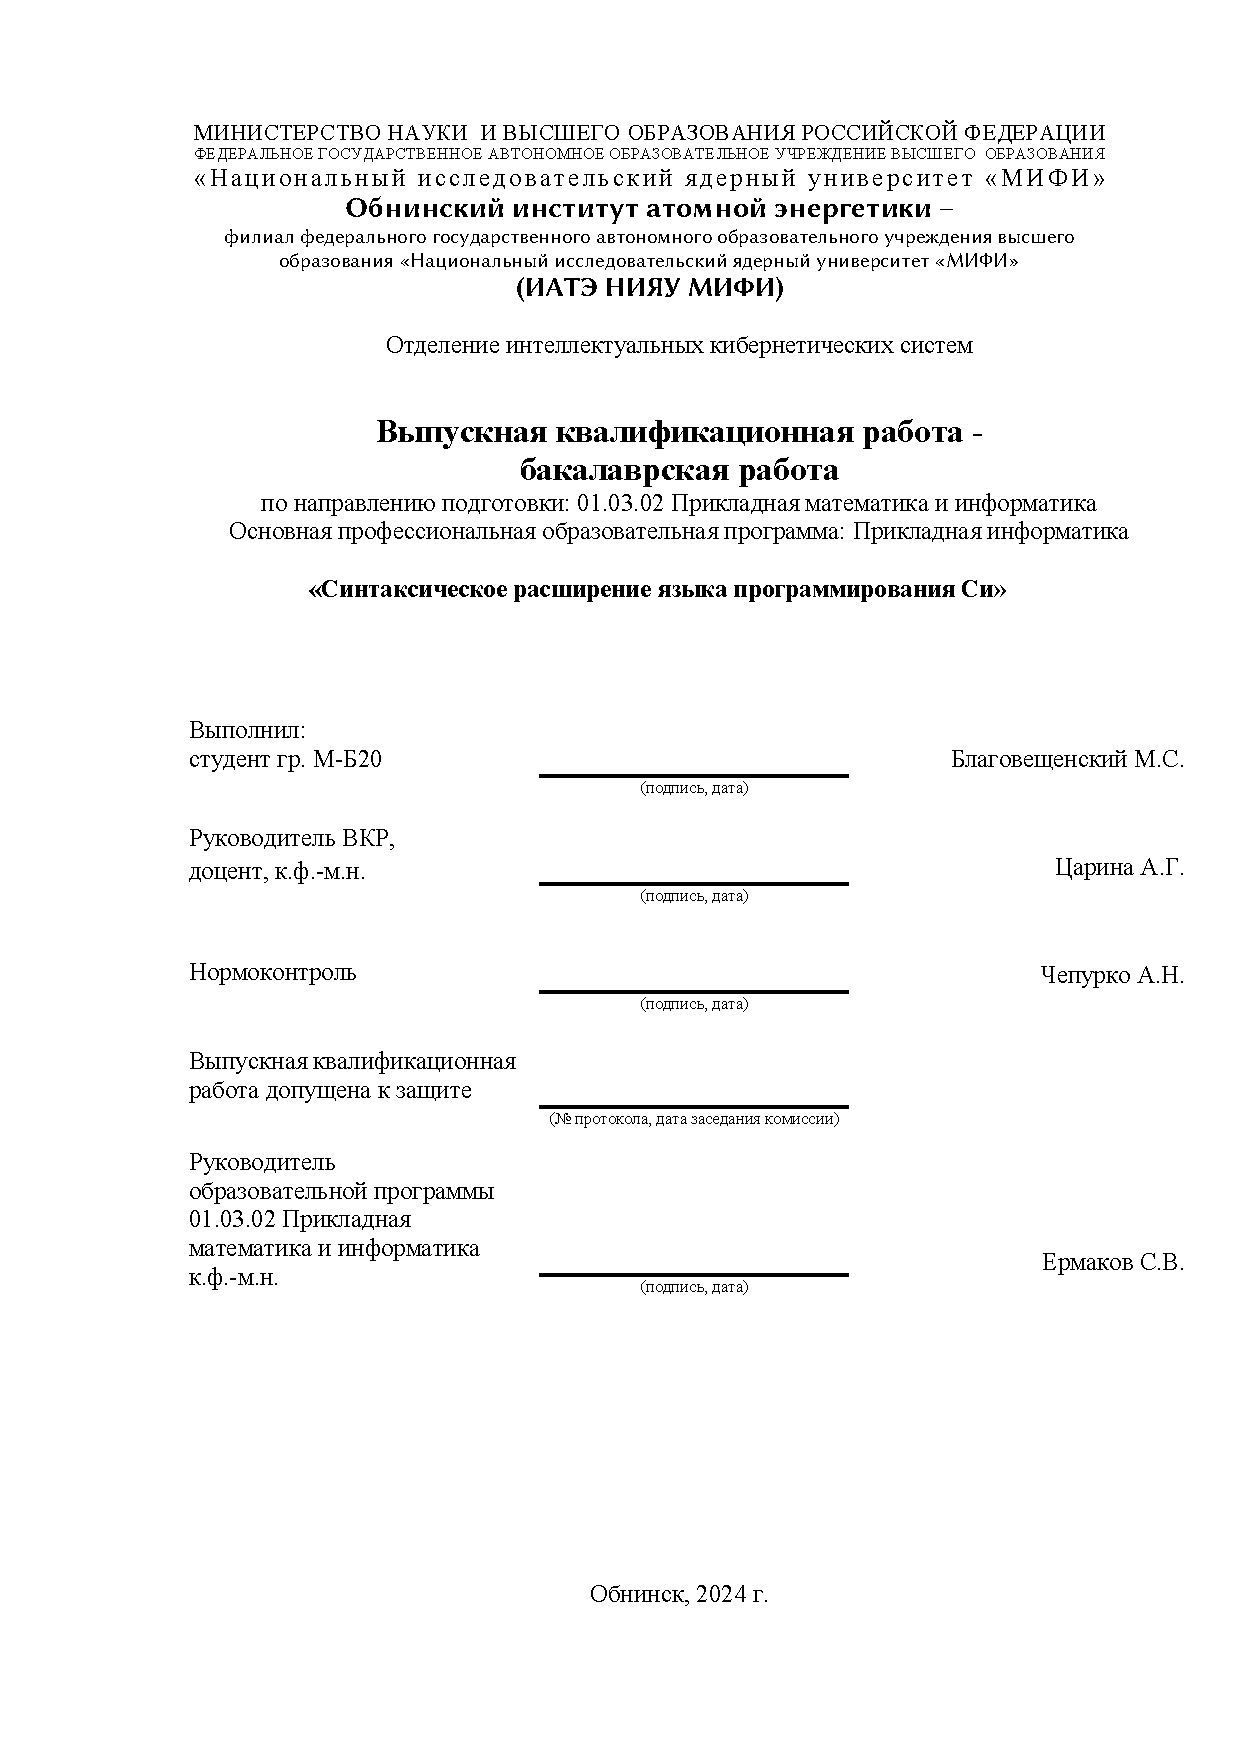
\includepdf[pages=-]{./extra/title_page.pdf}
           % Титульный лист
\pagenumbering{gobble} % без номера: введение
\chapter*{РЕФЕРАТ}
% \addcontentsline{toc}{chapter}{РЕФЕРАТ} 

% \begin{center}
Работа \formbytotal{TotPagesNoAppendix}{страниц}{у}{ы}{}, 
    \formbytotal{totalcount@figure}{рисун}{ок}{ка}{ков},
    % \formbytotal{totalcount@lstlisting}{листинг}{}{а}{ов},
    \formbytotal{totalappendix}{приложен}{ие}{ия}{ий},
    \formbytotal{citenum}{источник}{}{а}{ов}.
% \end{center}

    КОМПИЛЯТОРЫ, СИ, СИНТАКСИЧЕСКИЕ ДЕРЕВЬЯ, ГРАММАТИЧЕСКИЙ РАЗБОР, ПАРСИНГ, ЛЕКСИНГ, МАКРОСЫ, МЕТАПРОГРАММИРОВАНИЕ, ЯЗЫКИ ПРОГРАММИРОВАНИЯ. %\\[2pt]

    % \vspace{5mm}
% \paragraph*{Cтруктура работы.}
Данная работа посвящена разработке библиотеки грамматического разбора языка Си и разработке прототипа компилятора\break языка \textquote{Extended C} (\textquote{Расширенный Си}, далее \textquote{EC}) на основе этой библиотеки.

Объектом разработки является source-to-source компилятор \verb|ecc|, языка EC, являющейся небольшой надстройкой над языком Си.
Целью работы является совершенствование инструментария по работе с языком Си.

Задачами ВКР являются обзор и анализ существующих систем метапрограммирования в других языках, 
разработка аналогичной системы для языка EC,
демонстрация практической выгоды данной системы.

Новизна данной работы заключается в усовершенствовании устоявшегося языка Си.

Экономическая эффективность работы заключается в том, что реализованная в данной работе подсистема метапрограммирования позволяет, в некоторых случаях, значительно сократить работу программиста. %, что продемонстрировано[\ref{use-ex}]. % TODO ref

% \paragraph*{Структура работы.} 
Основная часть отчета состоит из двух частей:\\
Глава 1: обзор архитектуры проекта, примеры использования, сравнение его с решениями в других языках\\
Главы 2-5: рассмотрение деталей и алгоритмов работы компилятора

% \clearpage

% \begin{lstlisting}[language=c]
% @post_include("demo.h")

% @derive(DebugFormat)
% struct Foo {
%     int x;
%     int y;
%     int z;
% };

% int main() {
%     ctx_init_default();
%     print();
%     ctx_deinit();
% }

% void 
% print() {
%     Foo foo = (Foo) {
%         .x = 3,
%         .y = 4,
%         .z = 5,
%     };
%     dbgp(Foo, &foo);

% }
% \end{lstlisting}

% \clearpage
% \begin{lstlisting}[language=bash]
% $ ecc -p macro.ec example.ec -o example
% \end{lstlisting}

% \clearpage

% \begin{lstlisting}[language=bash]
% $ ./example
% Foo:
%     x: 3
%     y: 4
%     z: 5
% \end{lstlisting}

%% на случай ошибок оставляю исходный кусок на месте, закомментированным
%Полный объём диссертации составляет  \ref*{TotPages}~страницу
%с~\totalfigures{}~рисунками и~\totaltables{}~таблицами. Список литературы
%содержит \total{citenum}~наименований.
%
% Полный объём диссертации составляет
% \formbytotal{TotPages}{страниц}{у}{ы}{}, включая
% \formbytotal{totalcount@figure}{рисун}{ок}{ка}{ков} и
% \formbytotal{totalcount@table}{таблиц}{у}{ы}{}.
% Список литературы содержит
% \formbytotal{citenum}{наименован}{ие}{ия}{ий}.




% \newpage
% \section*{Основное содержание работы}

% В Главе~\ref{ch:ch1}... \pageref{extras:c_ast}

% \section*{Публикации автора по теме диссертации}


% Основные результаты по теме диссертации изложены в \theAllMyPapers~публикациях. 
% Из них
% %4 изданы в журналах, рекомендованных ВАК, 
% \theScopusPapers~опубликовано в изданиях, индексируемых в базе цитирования Scopus. 
% %Также имеется 1 свидетельство о государственной регистрации программ для ЭВМ.

% В международных изданиях, индексируемых в базе данных Scopus:
% \begin{refsection}[biblio/own.bib]
% \nocite{*}
% \printbibliography[
%     keyword=scopus,
%     %title={В международных изданиях, индексируемых в базе данных Scopus}, 
%     %heading=subbibliography,
%     heading=none,
%     resetnumbers=true
% ]
% \end{refsection}



% В международных изданиях, индексируемых в базе данных Web of Science:
% \begin{refsection}[biblio/own.bib]
% \nocite{*}
% \printbibliography[
%     keyword=wos,
%     %title={В международных изданиях, индексируемых в базе данных Web of Science}, 
%     %heading=subbibliography,
%     heading=none,
%     resetnumbers=true
% ]
% \end{refsection}
% Список всех публикаций автора по теме диссертации:
% \begin{refsection}[biblio/own.bib]
% \nocite{*}
% \printbibliography[
%     keyword=own,
%     %title={Список всех публикаций автора по теме диссертации}, 
%     %heading=subbibliography,
%     heading=none,
%     resetnumbers=true
% ]
% \end{refsection}
 % реферат на русском

% \setcounter{page}{2}    % оглавление начинается с 5 страницы, остальное генерится из ИСУ
\renewcommand{\figurename}{Рисунок}
\renewcommand{\tablename}{Таблица}
% \chapter*{Словарь терминов}             % Заголовок
\addcontentsline{toc}{chapter}{Словарь терминов}  % Добавляем его в оглавление

\textbf{TeX} : Cистема компьютерной вёрстки, разработанная американским профессором информатики Дональдом Кнутом

\textbf{панграмма} : Короткий текст, использующий все или почти все буквы алфавита
      % Словарь терминов

% Оглавление (ГОСТ Р 7.0.11-2011, 5.2)
\begingroup
    \ifdefmacro{\microtypesetup}{\microtypesetup{protrusion=false}}{} % не рекомендуется применять пакет микротипографики к автоматически генерируемому оглавлению
    % \setSpacing{0.9} 
    \setSpacing{1} 
    \tableofcontents*
    % \addtocontents{toc}{\protect\tocheader}
    \endTOCtrue
    \ifdefmacro{\microtypesetup}{\microtypesetup{protrusion=true}}{}
\endgroup        % Оглавление
% Если оч надо это автоматизировать, то смотри здесь
% https://www.overleaf.com/learn/latex/Nomenclatures
%\printnomenclature[3.5cm] % Значение ширины столбца с обозначениями стоит подбирать вручную

\chapter*{ОПРЕДЕЛЕНИЯ, ОБОЗНАЧЕНИЯ И СОКРАЩЕНИЯ}             % Заголовок
% \addcontentsline{toc}{chapter}{ОБОЗНАЧЕНИЯ И СОКРАЩЕНИЯ}  % Добавляем его в оглавление

% \newcommand{\acrstyle}[1]{\textbf{#1}}
\newcommand{\acrstyle}[1]{#1}


\acrstyle{Лексема(Токен)} - элементарная единица языка с точки зрения его грамматики. Может состоять из нескольких символов.
Примеры: ',' - запятая, '...' - троеточие, 'имя' - идентификатор, '"text"' - строковой литерал

\acrstyle{CFG} - Context-Free Grammar (контекстно-свободная грамматика)

\acrstyle{AST(АСД)} - Abstract Syntax Tree (абстрактное синтаксическое дерево)

\acrstyle{Лексер} - тип языка программирования, выполняющий лексический разбор

\acrstyle{Парсер} - тип языка программирования, выполняющий грамматический разбор


\acrstyle{Дерево} - связный граф, у каждого элемента которого не более одного предка

\acrstyle{Аллокатор} - абстрактный объект, предоставляющий интерфейс выделения/возврата памяти из кучи(heap)

\acrstyle{Стек(Stack)} -  структура данных, представляющий собой список элементов, организованных по принципу LIFO (last in — first out, последним пришёл — первым вышел).

\acrstyle{CLI} -  command line interface, интерфейс командной строки(терминала)

% Заранее ввожу следующие важные определения:

Метапрограмма - программа на некотором языке программирования, которая в процессе своей работы анализирует, трансформирует или генерирует код на том же или другом языке программирования.
Просты словами метапрограмма - программа, результатом работы которой является другая программа.

Метапрограммы это своего рода функции высшего порядка\cite{wiki-hof}, отображения между пространствами программ.

Метапрограммирование - процесс написания кода метапрограммы.        % Список сокращений и условных обозначений
\chapter*{Словарь терминов}             % Заголовок
\addcontentsline{toc}{chapter}{Словарь терминов}  % Добавляем его в оглавление

\textbf{TeX} : Cистема компьютерной вёрстки, разработанная американским профессором информатики Дональдом Кнутом

\textbf{панграмма} : Короткий текст, использующий все или почти все буквы алфавита
        
\pagenumbering{arabic}

\setcounter{page}{3}    % введение с 3й страницы
\ifnumequal{\value{contnumfig}}{1}{}{\counterwithout{figure}{chapter}}
\ifnumequal{\value{contnumtab}}{1}{}{\counterwithout{table}{chapter}}
% \renewcommand{\figurename}{Рисунок}
% \renewcommand{\tablename}{Таблица}

\chapter*{ВВЕДЕНИЕ}                         % Заголовок
\addcontentsline{toc}{chapter}{ВВЕДЕНИЕ}    % Добавляем его в оглавление

% Заранее ввожу следующие важные определения:

% Метапрограмма - программа на некотором языке программирования, которая в процессе своей работы анализирует, трансформирует или генерирует код на том же или другом языке программирования.
% Просты словами метапрограмма - программа, результатом работы которой является другая программа.

% Метапрограммы это своего рода функции высшего порядка\cite{wiki-hof}, отображения между пространствами программ.

% Метапрограммирование - процесс написания кода метапрограммы.
% \newline
% \vspace{5pt}
% \section*{Актуальность проблемы}
% \section*{}
Язык программирования - основной инструмент любого разработчика. От его эргономики, то насколько легко на нем излагать идеи, напрямую зависит продуктивность разработчика, а также его эмоциональное состояние.

В случае языка Си необходимость линейно упорядочивать определения, вызванная ограничениями по ресурсам вычислительных устройств того времени, когда он был разработан, 
и отсутствие функционала метапрограммирования, понижают его эргономику.

Цель данной работы - повышение эргономики и модернизация языка Си.

% На практике часто встречаются задачи, когда стандартных утилит для работы с языком недостаточно, и приходится писать свои собственные. 
% Например в вашем проекте оптимизац
% Другая цель данного проекта - помочь в разработке подобных утилит, путем предоставления модифицируемого source-to-source компилятора.

Идея состоит в том, чтобы часть функционала компилятора Си, вынести в виде пользовательской библиотеки, с возможность ее модифицирования и доработки. 
Это позволяет разработчику процедурно обрабатывать код, что открывает возможность создания автоматизированных систем по работе с кодом.

Пример такой системы реализован в данной работе с применением синтаксического расширения языка Си, добавляющего \textquote{@ директивы}.

Далее язык Си вместе с автоматизированной системой буду называть просто \textquote{Расширенный Си} (англ. \textquote{Extended C}, сокр. \textquote{EC}). 
% Необходимость такого функционала возникает, когда у разработчика возникает потребность процедурно обрабатывать код

% Си устоявшийся(stable) и стандартизированный язык, 
% поэтому нет проблемы нестабильного API из-за постоянно развивающего языка.%, как например сейчас происходит в Rust.

% Разработчику предлагается использовать данную библиотеку для превращения программного кода в абстрактное синтаксическое дерево - 
% структуру данных, которая может быть обработано процедурно (программным путем).

% Библиотека ec может быть использована отдельно от компилятора ecc для написания своих собственных утилит для работы с языком Си.

В данной работе представлен source-to-source компилятор языка EC - \textquote{Extended C Compiler} (сокр. ecc), представлющий по своей сути слой предобработки исходного кода языка Си, 
с дополнительным функционалом интерпретации директив синтаксического расширения. 




% \section*{Постановка задачи}
Задачами данной выпускной квалификационной работы являются:

\begin{itemize}
    \item Изучение стандартов\cite{c99_std}\cite{c23_std} языка Си
    \item Разработка AST для языка Си по его CFG, написание библиотеки грамматического разбора языка Си
    \item Проектирование синтаксического расширения языка Си
    \item Разработка прототипа компилятора языка EC
    \item Разработка системы макросов для языка EC
\end{itemize}

% \textbf{ecc} является source-to-source компилятором, т.е.компилятором, транслирующих текст программы на одном языке программирования в текст программы 
% на другом (возможно том же самом) языке программирования. 
% В данном случае после разбора текста синтаксическая надстройка на Си интерпретируется, после чего полученное в ходе интерпретации дерево компилируется к тексту языка Си.


% TODO add ref

% \clear
В процессе работы в процессе работы были разобраны следующие источники:

\newcommand{\titlecite}[1]{\citetitle{#1}\cite{#1}}

\titlecite{c23_std}, \titlecite{c99_std} - основные документы, содержащие информацию о языке Си.
В основном использовалась грамматика языка, которая подытожена в Annex A, данных нормативных документов. 
Также использовалась информация о стадиях и порядке трансляции.

\titlecite{crafting_interpreters} - основная книга, использованная в данной работе. 
В ней продемонстрирован метод рекурсивного спуска, описан лексер и парсер для придуманного автором языка Lox.
На основе главы этой книги была написана имплементация хэш-таблицы, использованной в данной работе[\ref{primitives:hashmap}].

\titlecite{hmu} - теория формальных языков, абстрактных вычислительных машин и грамматик. 
Данная книга использовалась как источник математического знания по теме на ранних этапах изучения.

\titlecite{dragon_book} - классическая так называемая \textquote{Книга Дракона}, использовалась на ранних стадиях изучения предметной области для ознакомления с темой.

The Theory of Parsing, Translation, and Compiling (Volume I, II)
\cite{ptc_vI} \cite{ptc_vII} - классические книги по теории компиляции.

\titlecite{monparsing_paper}, \titlecite{ml_syntax_transformation_paper} - статьи про монадические парсеры, рассматривались на ранних стадиях прототипирования парсера.

\titlecite{peg_paper} - оригинальная статья автора PEG грамматики, 
рассматривалась при изучении видов грамматик и парсер-генераторов для грамматик формальных языков.
PEG - Parsing expression grammar, тип аналитической формальной грамматики, является аналогом CFG. 
Однако благодаря свойствам детерминированного оператор выбора в данном формализме в отличие от CFG PEG не может быть неоднозначной, 
т.е. если дерево разбора для грамматики PEG существует, то оно единственное.

\titlecite{parsing_techniques} - при изучении PEG грамматики была рассмотрена глава 15.7 \textquote{Recognition Systems} данной книги.

Были рассмотрены следующие источники по теме \textquote{Разбор выражений и приоритет операций}:
% \subsection*{Разбор выражений и приоритет операций}

% \caption{pratt}
% \label{litover:pratt} \mbox{} \\
\titlecite{tdop_pratt_paper} - оригинальная статья автора парсера Пратта, использовалась для ознакомления с темой.

\titlecite{matklad_pratt_parsers} - из этой статьи позаимствована идея конкретной имплементация парсера Пратта.

\titlecite{cppref_op_prec} - справка по языку Си: приоритет операций, использовалась при построении таблицы[\ref{extras:c_defs}] приоритетов операций.

\titlecite{pest_op_pratt} - парсер Пратта в фреймворке pest.

При разработке парсера были рассмотрены синтаксические деревья и методы грамматического разбора в других языках:

В языке Rust абстрактное синтаксическое дерево\cite{rust-ast} выполнено средствами богатой системы типов Rust, 
такими как энумерации(\verb|enum|), которые в Rust могут выполнять функцию помеченных объединений(tagged unions).
Функционал, доступный под ключевым словом \verb|match|, проверяет, чтобы все под-элементы данного элемента AST были обработаны,
что значительно снижает кол-во ошибок при работе с AST. В данной работе за неимением подобных проверок в Си используются 
функции \textquote{заглушки} \verb|unreachable| и \verb|unimplemented|, рассмотренные далее[\ref{primitives}].

Был рассмотрен парсер Rust\cite{rustc-parser}.
Структура, полученная в ходе лексического разбора кода Rust является вложенной, поэтому в парсере используется стек для итерации по данной структуре.
В данной работе я отказался от использования стека и решил уплощить структуру.


Был рассмотрен язык Odin. Была рассмотрена часть его стандартной библиотеки, отвечающая за его синтаксический разбор и анализ\cite{odin-parser}.
Стандартная библиотека языка Odin служила хорошим примером при разработке библиотеки примитивов[\ref{extras:c-core}]

Было рассмотрено синтаксическое дерево языка Python\cite{python-ast} и интерфейс позволяющий работать с ним. 
Python использовался для изучения AST структуры на этапе изучения предметной области.


Была рассмотрена система генерации \verb|go generate| языка Go, описанная в статье \titlecite{go-gen}.
Данная система рассматривалась совместно с модулями AST\cite{go-ast} и грамматического разбора\cite{go-parser} языка Go.
Следующая статья содержит множество полезных примеров использования данной системы: \titlecite{go-tool-guide}.

Был рассмотрен язык Julia, система метапрограммирования\cite{julia-meta}, 
синтаксически похожая на систему выполненную в данном проекте, подробнее далее[\ref{langcmp:julia}]. 

Был рассмотрен язык Zig и его \verb|comptime| функционал\cite{zig-comptime}.
На основе примеров приведенных в стандартной библиотеке языка Zig были разработаны интерфейс аллокатора[\ref{primitives:allocator}] и виртуальные таблицы для динамических интерфейсов.









% \paragraph*{Актуальность темы.}


% \paragraph*{Цель работы.}

% \paragraph*{Задачи работы.}

% \paragraph*{Научная новизна работы.}

% \paragraph*{Теоретическая и практическая значимость работы.}

% \paragraph*{Положения выносимые на защиту.}
% \begin{enumerate}
%     \item \statementOneRU
%     \item \statementTwoRU 
% \end{enumerate}

% \paragraph*{Апробация работы.}

% \paragraph*{Достоверность научных достижений.}

% \paragraph*{Внедрение результатов работы.}

% \paragraph*{Публикации.} Список всех публикаций автора по теме диссертации:
% \begin{refsection}[biblio/own.bib]
% \nocite{*}
% \printbibliography[
%     keyword=own,
%     %title={Список всех публикаций автора по теме диссертации}, 
%     %heading=subbibliography,
%     heading=none,
%     resetnumbers=true
% ]
% \end{refsection}



% \paragraph*{Структура и объем диссертации. }
% Диссертация состоит из~введения,
% \formbytotal{totalchapter}{глав}{ы}{}{},
% заключения и
% \formbytotal{totalappendix}{приложен}{ия}{ий}{}.
% %% на случай ошибок оставляю исходный кусок на месте, закомментированным
% %Полный объём диссертации составляет  \ref*{TotPages}~страницу
% %с~\totalfigures{}~рисунками и~\totaltables{}~таблицами. Список литературы
% %содержит \total{citenum}~наименований.
% %
% Полный объём диссертации составляет
% \formbytotal{TotPages}{страниц}{у}{ы}{}, включая
% \formbytotal{totalcount@figure}{рисун}{ок}{ка}{ков} и
% \formbytotal{totalcount@table}{таблиц}{у}{ы}{}.
% Список литературы содержит
% \formbytotal{citenum}{наименован}{ие}{ия}{ий}.


% \begin{figure}
%     \centering
%     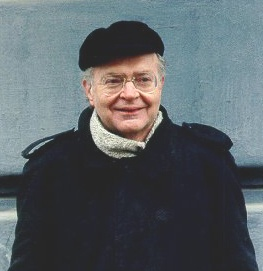
\includegraphics[width=0.6\linewidth]{images/knuth}
%     \caption{Knuth}
%     \label{fig:my_label}
% \end{figure}    % Введение


\ifnumequal{\value{contnumfig}}{1}{\counterwithout{figure}{chapter}
}{\counterwithin{figure}{chapter}}
\ifnumequal{\value{contnumtab}}{1}{\counterwithout{table}{chapter}
}{\counterwithin{table}{chapter}}

%%% В основном тексте выравниваем главы по параграфу
\makeatletter
\makechapterstyle{thesisgostchapname}{%
	\chapterstyle{thesisgost}
	\renewcommand*{\printchapternum}{\chapnumfont \thechapter}
	\renewcommand*{\printchaptername}{\hdngalign\chapnamefont \@chapapp} %
}
\makeatother
\chapterstyle{thesisgost}

\ifnumequal{\value{chapstyle}}{1}{%
	\chapterstyle{thesisgostchapname}
	\renewcommand*{\cftchaptername}{\chaptername\space} % будет вписано слово Глава перед каждым номером раздела в оглавлении
}{}%
%%%

\chapter{ОБЗОР ПРОЕКТА}
\label{ch:ch1}


\section{Архитектура проекта}

Требования к окружению для текущего прототипа:
\begin{itemize}
\item OS: GNU/Linux
\item Наличие компилятора gcc
\end{itemize}

\vspace{5pt}
Проект выполнен как динамическая библиотека \verb|libec.so| и небольшая утилита \verb|ecc| использующая ее.

Следующая диаграмма[\ref{arch:diag}] иллюстрирует архитектуру проекта:

\begin{figure}[h!]
    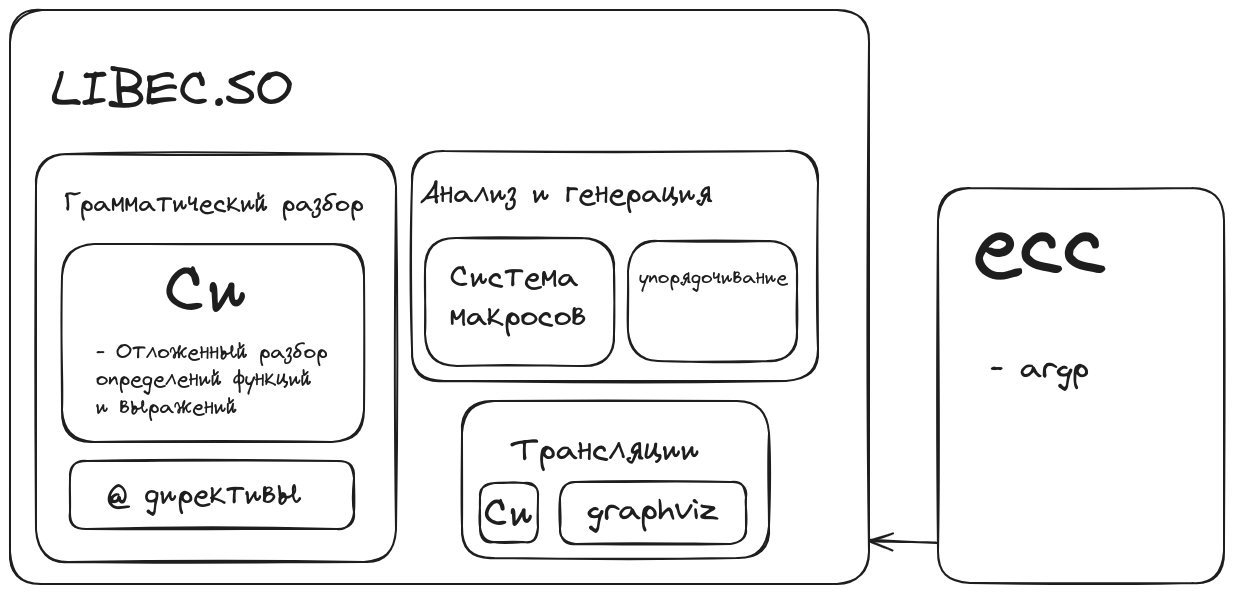
\includegraphics[width=\textwidth,height=0.8\textheight,keepaspectratio]{arch-diag.png}
    \centering
    \caption{Архитектура проекта}
    \label{arch:diag}
\end{figure}

Библиотека \verb|ec.so| имеет высокоуровневый интерфейс, реализованный в виде методов единицы трансляции(в коде \verb|C_TranslationUnitData|).
Данный интерфейс организует функционал библиотеки в виде проходов и их композиций.
Каждый проход это отдельный этап трансляции. 
Подробно каждый проход рассматривается в следующей главе[\ref{passes}].

Так как синтаксически ЕС это небольшая надстройка над языком Си, 
то парсер Си(и некоторые другие проходы, например трансляции) библиотеки ec.so может быть использован отдельно от языка EC.

Интерфейс утилиты \verb|ecc| подробно описан далее[\ref{details:ecc-cli}].

% Данный функционал предоставлен пользователю для решения задач метапрограммирования: предобработки, умной компиляции, и др.

% Поверх стандартного функционала разбора языка Си в библиотеку добавлено синтаксическое расширение языка: Extended C
% Которое может быть использовано пользователем для разметки программного кода с целью последующей его обработки, что продемонстрировано далее[\ref{use-ex:code-gen}]

\section{Обзор языка EC}

EC представляет собой слой предобработки языка Си, повышающий его эргономику.
EC реализует систему директив, выполняющих функцию разметки кода, с возможностью последующей их интерпретации.

В реализованном на данный момент прототипе представлены следующие директивы:
\begin{itemize}
\item \verb|@derive(identifier)| применяет к следующему за директивой определению макро-функцию вывода указанную в \verb|identifier|
\item \verb|@derive_macro(identifier)| регистрирует следующее за директивой определение функции как макро-функцию вывода адресуемую с помощью \verb|identifier|
\item \verb|@post_include(string-literal)| при трансляции в язык Си заменяется на обычную директиву препроцессора \verb|#include string-literal|
\end{itemize}

С помощью данных директив в EC реализованна система макросов. На данный момент реализованны только макросы вывода (derive macro).
Макросы(или макро-функции) вывода это функции, генерирующие блок кода, оформленного в виде элемента AST единицы трансляции, по данному AST определению.

Все макро-функции вывода должны иметь следующий интерфейс:
\begin{lstlisting}[language=C]
typedef ProcMacroError
DeriveMacroFn(C_TranslationUnitData *, C_Ast_Decl *, C_Ast_TranslationUnit **);
\end{lstlisting}

Макро-функции должны находиться в отдельном файле, т.к. библиотека макро-функций является отдельной единицей трансляции.
При компиляции \verb|ecc| сначала компилирует все макро-функции как динамическую библиотеку, линкуя ее с основной библиотекой \verb|libec.so|, затем динамически подгружает ее в свое виртуальное адресное пространство, после чего возможен вызов данных функций.
Подробнее этот процесс описан далее[\ref{pass:macros}].

Зачастую бывает нецелесообразно генерировать код заполняя AST структуру вручную, альтернативой этому на данный момент служит написание генерируемого кода в виде строки,
используя вспомогательный примитив \verb|StringFormatter|, рассмотренный далее[\ref{primitives:formatter}], и последующий его грамматический разбор.
Функционал грамматического разбора, приведенный в заголовочном файле \verb|proc_macro.h| использует библиотеку \verb|libec.so|.

Рассмотрим пример макро-функции вывода:
\lstinputlisting[language={C},caption={macros.ec},label={use-ex:macro-file}]{listings/ch1/use-ex/ex_macro.ec}

Данная макро-функция генерирует функции отладочного форматирования для структур языка Си.
Вспомогательная функция \verb|gen_dbg_fmt_fmt| генерирует текст программы, а основная выполняет функцию обработки ошибок и грамматического разбора текста сгенерированной программы.
Получившийся в процессе генерации AST элемент(единица трансляции) возвращается компилятору, выполняющему дальнейшие преобразования.

Так например из следующего определения структуры языка Си
\begin{lstlisting}[language=C]
struct Foo {
    int x;
    int y;
    int z;
};
\end{lstlisting}

генерируется следующая функция отладочного форматирования
\begin{lstlisting}[language=C]
FmtError Foo_dbg_fmt(Foo *self, StringFormatter *fmt, void *_) {
    TRY(string_formatter_write_fmt(fmt, S("Foo:%+\nx: %d\ny: %d\nz: %d\n%-"), self->x, self->y, self->z));
    return FMT_ERROR(OK);
}
\end{lstlisting}

печатающая структуру \verb|Foo| со значениями полей: \verb|x=3, y=4, z=5| следующим образом
\begin{lstlisting}[language=C]
Foo:
    x: 3
    y: 4
    z: 5
\end{lstlisting}

В примере[\ref{use-ex:macro-file}] функция \verb|gen_dbg_fmt| помечена директивой \verb|@derive_macro(DebugFormat)|, регистрирующей ее в базе макро-функций компилятора под именем \verb|DebugFormat|.
Далее данная функция может быть применена к определению языка Си с помощью родственной директивы \verb|@derive(DebugFormat)|.

Пример использования данной макро функции приведен далее[\ref{use-ex:code-gen}].

\section{Пример программы на EC}
\label{use-ex:simple}

Для демострации языка приведем следующую простую программу[\ref{use-ex:simple-souce}]:
\begin{lstlisting}[language=C, caption={simple.ec}, label={use-ex:simple-souce}]
@post_include("demo.h")

struct A {
    B b;
};

int main() {
    ctx_init_default();
    
    g_x = 5;
    foo(g_x);

    ctx_deinit();
}

struct B {
    A *ap;
    C c;
};
struct C {
    B *bp;
};

int g_x;

void foo(int x) {
    print_fmt(S("x: %d\n"), x);
}
\end{lstlisting}

Данная программа не скомпилируется компилятором Си, даже если заменить директиву в начале файла на обычный \verb|#include "demo.h"|.
Так например \verb|gcc| выдает ошибку[\ref{use-ex:simple-gcc-err}]:

\begin{lstlisting}[language=Bash, caption={Ошибка gcc}, label={use-ex:simple-gcc-err}]
error: unknown type name ‘B’
...
error: ‘g_x’ undeclared
...
\end{lstlisting}

Связано это с тем, что в Си зависимости разрешаются линейно(сверху вниз), 
т.е. когда компилятор увидел имя \verb|B| в структуре \verb|A| он \textquote{запаниковал}, так как ранее(выше) это имя не приводилось.

В EC внешние определения могут идти в любом порядке. Под внешними в данном случае понимается те, 
что приведены непосредственно в корне файла, не содержатся в определении функции(или составного утверждения).

Также в примере используются \textquote{голые} имена структур, тогда как в Си при объявление, 
приведенном в примере, имена структур(и других составных типов) надо приводить с префиксом, например \verb|struct A|.
EC избавляет пользователя от данной необходимости.
% EC вставляет \verb|typedef struct A A;| в генерируемый Си файл, что объ

Подробнее об ток, как EC преобразует внешние определения см. далее[\ref{pass:ordering}].

Скомпилируем данную программу компилятором \verb|ecc| с помощью команды:
\begin{lstlisting}[language=Bash]
$ ecc simple.ec -o simple
\end{lstlisting}

Запуская полученный файл, получаем ожидаемый результат:
\begin{lstlisting}[language=Bash]
$ ./simple
x: 5
\end{lstlisting}


\section{Пример генерации кода}
\label{use-ex:code-gen}

Продемонстрирую как выглядит процесс работы с системой макросов языка EC.

Допустим у вас есть файл[\ref{use-ex:source-file}] \verb|example.ec| с исходным кодом EC, который вы хотите скомпилировать, предварительно применив макро-функции, определенные по требованиям системы макросов в отдельном файле, назовем \verb|macros.ec|.
Пусть содержание файла совпадает с приведенном ранее в обзоре языка EC[\ref{use-ex:macro-file}].

% \lstinputlisting[language={C},caption={example.ec},label={use-ex:source-file}]{listings/ch1/use-ex/ex4.ec}
\begin{lstlisting}[language=c, caption={example.ec}, label={use-ex:source-file}]
@post_include("parsing/c/parsing.c")

@derive(DebugFormat)
struct Foo {
    int x;
    int y;
    int z;
};

@derive(DebugFormat)
struct Bar {
    int x;
    int y;
    int z;
};

int main() {
    ctx_init_default();

    Foo foo = (Foo) {
        .x = 3,
        .y = 4,
        .z = 5,
    };
    dbgp(Foo, &foo);

    Bar bar = (Bar) {
        .x = 6,
        .y = 7,
        .z = 8,
    };
    dbgp(Bar, &bar);

    ctx_deinit();
}
\end{lstlisting}

Данный файл состоит из определений двух структур(\verb|Foo| и \verb|Bar|), для которых автоматически генерируются функции отладочного форматирования посредством директивы \verb|@derive|.
С помощью макроса препроцессора Си \verb|dbgp|, подхватывающего данные функции форматирования, печатаем в консоль значения содержащиеся в структурах.

Итак содержимое файла \verb|example.ec| компилирует с применение макросов командой:
\begin{lstlisting}[language=Bash]
$ ecc -p macro.ec example.ec -o example
\end{lstlisting}

Запуская полученный файл, получаем напечатанные структуры:
\begin{lstlisting}[language=Bash]
$ ./example
Foo:
    x: 3
    y: 4
    z: 5

Bar:
    x: 6
    y: 7
    z: 8
\end{lstlisting}

В этом примере используются всего две структуры, когда кол-во подобных объектов возрастает, возрастает и эффективность данной системы.

Результат работы данной системы можно увидеть, если посмотреть сгенерированный промежуточный файл[\ref{use-ex:c-tmp}] с кодом языка Си.

\lstinputlisting[language={C},caption={example\_tmp.c},label={use-ex:c-tmp}]{listings/ch1/use-ex/ex4_tmp.c}

Подробнее данный процесс будет рассмотрен далее[\ref{pass:ordering}, \ref{pass:macros}]

\section{Сравнение с другими языками}
Рассмотрим решения в других языках программирования:

\begin{enumerate}
% \item\label{langcmp:c} Сравнение с языком C:\brake - line was streched
\item\label{langcmp:c} Сравнение с языком C:\newline
Си - довольно старый системный язык, разработанный Деннисом Ритчи еще в 70х годах прошлого столетия, однако активно применяется и по сей день, среди ярких примеров применения: ядро операционной системы Linux, различные embedded системы.
С тех пор вышло несколько версий языка, среди них самая последняя C23, она же использовалась при написании данной работы.
Си это язык со слабой статической типизацией, благодаря чему во многом представляет собой высокоуровневый ассемблер.

В данной работе реализованно небольшое синтаксическое расширение языка Си, представляющее собой своеобразную систему разметки, семантическая часть языка не тронута.
Улучшена эргономика языка за счет автоматического упорядочивания определений(структурный элементов языка) в порядке зависимостей, что было продемонстрировано выше[\ref{use-ex:simple}].



\item\label{langcmp:cpp} Сравнение с языком C++:\newline
C++ является системным языком программирования, доминирующим на рынке в сфере ПО с требованиями по производительности. 
C++ несомненно объемный язык, в нем присутствуют такие системы как:
\begin{itemize}
\item подмножество языка Си
\item расширенная система типов Си
\item статический полиморфизм на перегрузке функций
\item система шаблонов, которая применяется как для статического полиморфизма, так и для метапрограммирования
\item система пространств имен
\item ООП система с возможностями динамического полиморфизма
\end{itemize}

Все это многообразие делает процесс разрешения имен в C++ очень сложным. 
Некоторые системы C++, например система виртуальных функций, через которые реализуется динамический полиморфизм, 
не дают пользователю контроля на тем как именно виртуальные таблицы располагаются в памяти.

В тех случаях когда этот контроль важен(например при динамической подгрузке и линковке библиотек) зачастую вовсе отказываются данной подсистемы и реализуют аналогичную в стиле Си остальными средствами языка C++.

В философии EC подобные подсистемы должны быть реализованы в виде пользовательских библиотек, с улучшенной эргономикой посредством макросов, позволяющей расширять язык средствами самого языка.
Так разработчик имеет максимальный контроль над используемыми инструментами, неограничен в их доработке и настройке под конкретный проект.

Так как Си является частичным подмножеством языка C++, то пункты приведенные выше[\ref{langcmp:c}] также применяются.

Для C/C++ существует компилятор Clang, у которого frontend вынесен в качестве библиотеки, однако данный компилятор заточен больше на C++, что существенно усложняет Ast, 
поэтому было принято решения написать свой минималистичный frontend для Си.



\item\label{langcmp:rust} Сравнение с языком Rust:\newline
Rust является системным языком программирования с развитой системой типов, позволяющей проводить глубокий статический анализ, в частности анализ и выведение времени жизни переменных, 
что используется при обнаружение ошибок связанных с владением памятью, таких как
\begin{itemize}
\item использование после освобождения памяти(use-after-free)
\item повторное освобождение памяти(double-free) 
\item утечка памяти(memory-leak)
\end{itemize}


В языке Rust представлена система\cite{rust-proc-macro} процедурных макросов, схожая с системой, выполненной в данной работе.
В Rust также есть \verb|Derive| макросы(макросы вывода) дающие такой же функционал, что и \verb|@derive| директивы представленные в данной работе.
Макросы в Rust также компилируются в отдельной единице трансляции(\verb|crate| в терминологии Rust).

Отличие состоит в том, что макросы в Rust работают на уровне токенов(лексем), тогда как макросы в данном проекте работают на уровне элемента AST подобно языку Julia[\ref{langcmp:julia}].

Для сравнения привожу заголовки функций макросов из обоих языков[\ref{langcmp:rust:rust_pmh}, \ref{langcmp:rust:ec_pmh}]:


\begin{lstlisting}[language=C, caption={Заголовок процедурного макроса Rust}, label={langcmp:rust:rust_pmh}]
#[proc_macro_derive(AnswerFn)]
pub fn derive_answer_fn(_item: TokenStream) -> TokenStream;
\end{lstlisting}

\begin{lstlisting}[language=C, caption={Заголовок процедурного макроса EC}, label={langcmp:rust:ec_pmh}]
@derive_macro(DebugFormat)
ProcMacroError
gen_dbg_fmt(C_TranslationUnitData *data, C_Ast_Decl *decl, C_Ast_TranslationUnit **out_node);
\end{lstlisting}

Где \verb|TokenStream| - тип потока токенов в языке Rust.

Генерация кода, путем заполнения AST напрямую - трудоемкий и нецелесообразный подход.
Поэтому в Rust есть функционал "цитирования" кода, предоставляемый пакетом(\verb|crate|) \verb|quote|\cite{rust-quote}.
Данный пакет предоставляет макро-функцию \verb|quote!|, реализованную как декларативный макрос(еще один вид макросов) самого языка Rust.

Пример цитирования кода:
\begin{lstlisting}[language=C, caption={Заголовок процедурного макроса Rust}, label={langcmp:rust:rust_quote}]
let varname = format_ident!("_{}", ident);
quote! {
    let mut #varname = 0;
}
\end{lstlisting}

Так мы можем писать генерируемый код, как если бы писали код обычной функции. К тому же есть возможность подстановки выражений из локальных переменных.
Опять же все это работает на уровне токенов, т.е. макро-функция \verb|quote| возвращает поток токенов, получая блок текста(программы).

В моей работе на данный момент единственный целесообразный способ генерации кода это генерация его в виде строки, с последующим грамматическим разбором, как показано ранее в примере[\ref{use-ex:code-gen}].

Также в EC макро-функциях на вход приходит разобранный AST элемент, тогда как в Rust приходит простой поток токенов.
Для анализа и обработки программы нужно грамматически разобрать его, для этого в Rust есть пользовательский пакет \verb|syn|\cite{rust-syn}, реализующий парсер языка Rust.

Также как в EC порядок следования определений в тексте программы не играет роли в Rust.

\item\label{langcmp:julia} Сравнение с языком Julia:\newline
Язык Juila это скриптовый язык с динамической типизацией подобно языку Python. Система JIT(just-in-time, точно в срок)-компиляции, использующая LLVM\cite{llvm} позволяется данному языку компилироваться напрямую в машинный код, 
что благодаря оптимизациям LLVM позволяет добиться производительности близкой к производительности языка Си.

Язык Julia имеет похожую систему макро-функций\cite{julia-meta}, с единственным отличием, что в Julia макро-функции могут идти вперемешку с остальными. 
Связано это с тем, что в Julia определения функций интерпретируются линейно по ходу текста программы, в EC определения интерпретируются вне зависимости от порядка их следования в тексте.

Синтаксически макросы в Julia почти полностью совпадают с директивами EC.

\item\label{langcmp:zig} Сравнение с языком Zig:\newline
Zig это относительно молодой язык программирования, стремящийся занять туже нишу, что C/C++. 
Также как в Rust продвинутая система типов позволяет этому языку предотвратить множество ошибок при работе с памятью на этапе компиляции.
Если ставить в соответствие Zig, Rust и C, C++, то Zig будет ближе к C, а Rust будет ближе к C++.

В языке Zig метапрограммирование выполнено с помощью функционала \verb|comptime| - позволяющего выполнять код во время компиляции и функционала рефлексии, 
позволяющего получить информацию о типе в виде \verb|comptime| структуры, что предоставляет гибкий интерфейс для расширения возможностей компилятора, не прибегая 
к сторонним утилитам, а также для метапрограммирования, не взаимодействуя с AST напрямую.
\end{enumerate}           % Глава 1
\chapter{ДЕТАЛИ РЕАЛИЗАЦИИ}
\label{ch:ch2}

\section{Практическая часть: введение}

Разработана библиотека ec.so, в которой реализованны возможности source-to-source компилятора языка Си.
К этой библиотеке написана небольшая утилита \verb|ecc|, реализующая для нее cli интерфейс.

\subsection*{Интерфейс ecc}
Данная утилита(\verb|ecc|) является основным местом, куда пользователь идет при желании использовать компилятор.

\verb|ecc| использует библиотеку GNU argp для разбора и фильтрации аргументов, приходящих из командной строки. 
Argp автомачески генерирует сообщение[\ref{details:ecc-api:argp-usage-err}] об ошибке, при подаче неправильных аргументов.

\begin{lstlisting}[language=bash, caption={Пример сообщения об ошике, сгенерированного argp}, label={details:ecc-api:argp-usage-err}]
$ build/sandbox/ecc                                   
Usage: ecc [OPTION...] file...
Try `ecc --help' or `ecc --usage' for more information.
\end{lstlisting}

Так же argp добавляет ключ \verb|--help| и автоматически генерирует сообщение[\ref{details:ecc-api:argp-help}] со всеми основными ключами.
\begin{lstlisting}[language=bash, caption={Пример сообщения об использовании, сгенерированного argp}, label={details:ecc-api:argp-help}]
$ build/sandbox/ecc --help
Usage: ecc [OPTION...] file...
ecc - Extended C Compiler. Source-to-source compiler.

  -o, --output=FILE          Output to FILE instead of standard output
  -p, --proc-macro-file-path=<path>
                             Specify procedural macro file path
  -v, --verbose              Produce verbose output
  -?, --help                 Give this help list
      --usage                Give a short usage message
  -V, --version              Print program version

Mandatory or optional arguments to long options are also mandatory or optional
for any corresponding short options.
\end{lstlisting}

В случае успешного получения аргументов от \verb|arpg| \verb|ecc| далее просто вызывает соответвующие аргументам функции библиотеки \verb|ec|.


\subsection*{Структура компиляция языка}
Компиляция языка EC организована в виде последовательности проходов(passes), которые шаг за шагом преобразуют исходный текст программы в AST, 
трансформируют его, применяя макро-функции, переупорядочевая его, и транслируют в исходный код языка Си. 
Таким образом данный компилятор является sorce-to-source компилятором, т.к. преобразует исходный код одного языка к коду другого.

Проходы можно разделить на три группы:
\begin{itemize}
    \item Десериализирующие: к данной группе относятся проходы выводящие структуру из линейной последовательности элементов(символы, токены). 
    Сюда относятся проходы лексического[\ref{passes:lexing}] и грамматического разборов[\ref{passes:parsing}]
    \item Анализирующие и трансформирующие: к данной группе относятся проходы выполняющие манипуляции над AST деревом. 
    Сюда относятся проходы:
    \begin{itemize}
        \item Проход применения макросов[\ref{passes:macro-expansion}]
        \item Проход упорядочевания[\ref{passes:ordering}]
    \end{itemize}
    \item Сериализирующие: к данной группе относятся проходы уплощающие AST дерево в линейную последовательность элементов.
    Сюда относятся проходы:
    \begin{itemize}
        \item Проход трансляции в Си[\ref{passes:compile-c}]
        \item Проход трансляции в graphviz[\ref{passes:compile-dot}]
    \end{itemize}
\end{itemize}

В будующем планируется, что пользователь сможет добавлять свои проходы в процесс компиляции.

Далее в данной главе каждый из проходов будет рассмотрен в деталях.







Библиотека реализованна на языке C23, используется некоторые улучшения, добавленные в новом стандарте.

Используются:
\begin{enumerate}
  \item ключевое слово \textbf{auto} для автоматического вывода типов
  \item взятие адреса у литерала, например \verb|&(int) {3}|
  \item gcc выражения-утдверждения (statement expressions) вида \verb|({x = 3; x;})|
  \item gcc \verb|,##| оператор в макросах
\end{enumerate}


\subsection{Основные примитивы}
Для написания основной библиотки используюется дочерняя библиотека[\ref{extras:c-core}] с основными примитивами: 
строковыми, ввода-вывода, аллокации памяти и др.

Данная библиотека реализована в виде единичных самодостаточных заголовочных файлов, 
которые могут быть в зависимости от флага препроцессора либо заголовочными файлами либо файлами имплементации, 
по принципу stb библиотек\cite{stb_libs}.

% \subsubsection{Макросы}

% Для определений структур и энумераций используются следующие макросы:

% \beginminteddef{c}
% #define struct_decl(name) \
% typedef struct name name; \
% struct name; \

% #define enum_decl(name) \
% typedef enum name name; \
% enum name; \

% #define struct_def(name, fields) \
% typedef struct name name; \
% struct name fields; \

% #define enum_def(name, ...) \
% typedef enum name name; \
% enum name {__VA_ARGS__}; \
% \end{minted} 


% \subsubsection{Обработка ошибок}

% Ошибки кодируются как enum, например:

% \begin{listing}
% \caption{Ошибки Аллокатора}
% \beginminteddef{c}
% enum_def(AllocatorError,
%     ALLOCATOR_ERROR_OK,
%     ALLOCATOR_ERROR_MEM_ALLOC,
%     ALLOCATOR_ERROR_COUNT
% )
% #define ALLOCATOR_ERROR(ERR) ((AllocatorError)ALLOCATOR_ERROR_##ERR)
% \end{minted}
% \end{listing}

% Значение OK кодируется как 0, остальные значения кодируются положительными числами.

% Для обработки ошибок используются следующие макросы:
% % \begin{minted}[linenos, frame=single]{c}
% \beginminteddef{c}
% #define IS_OK(e) ({ \
%     auto _r = (e); \
%     *(int *)&(_r) == 0; \
%     })
% #define IS_ERR(e) ({ \
%     auto _r = (e); \
%     *(int *)&(_r) != 0; \
%     })
% #define TRY(expr) { \
%     auto _e_ = (expr); \
%     if (IS_ERR(_e_)) { \
%         return _e_; \
%     } \
%   }
% #define ASSERT(expr) \
%     if (!(expr)) { \
%         fprintf(stderr, "ASSERT at %s:%d:\n", __FILE__, __LINE__); \
%         panic(); \
%     } 
% #define ASSERTM(expr, msg) { \
%     if (!(expr)) { \
%         fprintf(stderr, "ASSERTM: %*s\nat %s:%d:\n", (int)(sizeof(msg)-1), msg, __FILE__, __LINE__); \
%         panic(); \
%     } \
% }
% #define ASSERT_OK(expr) { \
%     auto _e_ = (expr); \
%     if (IS_ERR(_e_)) { \
%         fprintf(stderr, "ASSERT_OK at %s:%d:\n", __FILE__, __LINE__); \
%         panic(); \
%     } \
% }
% \end{minted} 

% \verb|IS_OK|, \verb|IS_ERR| - проверяют была ли ошибка

% \verb|TRY| - если была ошибка верни ошибку из текущей функции 

% \verb|ASSERT_OK| - если была ошибка, критическое завершение программы 

% \subsubsection{Контекст}
% Используется глобальный контекст, уникальный для каждого потока:

% \beginminteddef{c}
% __thread struct {
%     Allocator global_alloc;

%     Arena imm_str_arena;
%     Allocator imm_str_alloc;
%     slice_T(u8_t) dump_buffer;

%     void (*raise)(Error);

%     StreamWriter stdout_sw;
%     StreamWriter stderr_sw;
% } g_ctx;
% \end{minted} 

% \subsubsection{Аллокатор}

Вдохновленно походом, предложенным в языке Zig, каждая функция выделяющая память принимает на вход абстрактный аллокатор,
что одновременно указывает на то, что функция может выделять память(является своеобразной разметкой), 
а также является гибким решением при работе с паматью.

% Используется интерфейс абстрактного аллокатора:

% \beginminteddef{c}
% AllocatorError
% allocator_alloc(Allocator* self, usize_t size, usize_t alignment, void **out_ptr);
% AllocatorError
% allocator_resize(Allocator* self, usize_t size, usize_t alignment, void **in_out_ptr);
% allocator_free(Allocator* self, void **ptr);

% AllocatorError
% allocator_alloc_z(Allocator* self, usize_t size, usize_t alignment, void **out_ptr);
% \end{minted} 

% Примерами такого аллокатора служат глобальный glibc аллокатор и арена алокатор 

% \subsubsection{Арена Памяти}
% Для оптимизации и удобства работы с памятью используется структура арены памяти.

% \beginminteddef{c}
% struct_def(ArenaChunk, {
%     u8_t *cursor;
%     usize_t data_size;
%     u8_t data[];
% })

% struct_def(Arena, {
%     list_T(ArenaChunk) chunks;
%     usize_t default_chunk_data_size;
% })
% \end{minted} 


% \subsubsection{Строки}
% Строки и строковые "срезы" (позразумевается, что \textit{String} владеет паматью, т.к. хранит абстрактный аллокатор, 
%  а \textit{str\_t} нет)

% \beginminteddef{c}
% struct_def(String, {
%     uchar_t *ptr;
%     usize_t byte_cap;
%     usize_t byte_len; // in bytes
%     Allocator allocator;
% })

% struct_def(str_t, {
%     uchar_t *ptr;
%     usize_t byte_len; // in bytes
% })

% typedef uint32_t rune_t;
% \end{minted}

% Подразумевается, что строки используют UTF-8 кодировку.

% Тип \verb|rune_t| - unicode code point, число кодирующее символ в стандарте Юникод.

% Интерфейс итераторов считывания/записи юникод символов:
% \beginminteddef{c}
% UTF8_Error
% str_next_rune(str_t self, rune_t *out_rune, str_t *out_self);

% /// @param[in, out] out_str should be preinit, len 4 guaranties success
% UTF8_Error
% str_encode_next_rune(str_t self, rune_t rune, str_t *out_self);
% \end{minted}


% \subsubsection{Потоки ввода вывода}

% Интерфейс абстрактного потока вывода:

% \beginminteddef{c}
% enum_def(IOError, 
%     IO_ERROR_OK,
%     IO_ERROR_WRITE,
% )
% #define IO_ERROR(ERR) ((IOError)IO_ERROR_##ERR)

% typedef IOError (StreamWriter_WriteFn)(void *, usize_t, uint8_t[]);
% typedef IOError (StreamWriter_FlushFn)(void *);

% struct_def(StreamWriter_VTable, {
%     StreamWriter_WriteFn *write;
%     StreamWriter_FlushFn *flush;
% })
% struct_def(StreamWriter, {
%     StreamWriter_VTable _vtable;

%     void *data;
% })
% \end{minted}

% Тип \verb|OutputFileStream| - поток вывода в файл, реализующий привиденный ранее интерфейс.

% \beginminteddef{c}
% struct_def(OutputFileStream, {
%     slice_T(u8_t) buffer;
%     void *b_cursor;
%     void *e_cursor;
%     FILE *file;
% })

% AllocatorError
% output_file_stream_new_in(FILE *ofile, usize_t buffer_size, Allocator alloc[non_null], OutputFileStream *out_self);
% IOError
% output_file_stream_write(OutputFileStream self[non_null], usize_t data_size, u8_t data[data_size]);
% IOError
% output_file_stream_flush(OutputFileStream self[non_null]);
% StreamWriter
% output_file_stream_stream_writer(OutputFileStream self[non_null]);
% \end{minted}

% Строки тоже реализуют этот интерфейс(приведено с имплементацией).

% \beginminteddef{c}
% IOError
% output_string_stream_write(String self[non_null], usize_t data_size, u8_t data[data_size]);
% IOError
% output_string_stream_flush(String self[non_null]);
% StreamWriter
% string_stream_writer(String self[non_null]);

% IOError
% output_string_stream_write(String self[non_null], usize_t data_size, u8_t data[data_size]) {
%     ASSERT_OK(string_reserve_cap(self, data_size));
%     ASSERT_OK(string_append_str(self, (str_t) {.ptr = data, .byte_len = data_size}));
%     return IO_ERROR(OK);
% }
% IOError
% output_string_stream_flush(String self[non_null]) {
%     return IO_ERROR(OK);
% }
% StreamWriter
% string_stream_writer(String self[non_null]) {
%     return (StreamWriter) {
%         ._vtable = (StreamWriter_VTable) {
%             .write = (StreamWriter_WriteFn *)output_string_stream_write,
%             .flush = (StreamWriter_FlushFn *)output_string_stream_flush,
%         },
%         .data = (void *)self,
%     };
% }
% \end{minted}


% Используются следующие коды, для изменения цвета текста, при вывод в терминал.
% \beginminteddef{c}
% #define KNRM  "\x1B[0m"
% #define KRED  "\x1B[31m"
% #define KGRN  "\x1B[32m"
% #define KYEL  "\x1B[33m"
% #define KBLU  "\x1B[34m"
% #define KMAG  "\x1B[35m"
% #define KCYN  "\x1B[36m"
% #define KWHT  "\x1B[37m"
% \end{minted}

% \subsubsection{Форматирование строк}

% Для форматирования строк используется тип \verb|StringFormatter|, содержащий текущее состояние форматирования и настройки форматирования:
% строку для индентации(например \verb|"    "|), выходной поток, куда форматтер выводит результат.

% \beginminteddef{c}
% enum_def(FmtError,
%     FMT_ERROR_OK,
%     FMT_ERROR_ERROR,
% )

% struct_def(StringFormatter, {
%     usize_t pad_level;
%     str_t pad_string;

%     StreamWriter target;

%     bool is_line_padded;
% })
% \end{minted}

% Основыные методы типа \verb|StringFormatter|:
% \beginminteddef{c}
% FmtError
% string_formatter_write(StringFormatter *fmt, const str_t s);
% FmtError
% string_formatter_writeln(StringFormatter *fmt, const str_t s);
% FmtError
% string_formatter_write_fmt(StringFormatter *fmt, str_t fmt_str, ...);
% \end{minted}

% Выше \verb|write_fmt| реализует функционал схожий с функций \verb|glibc| \verb|printf|, 
% добавлена поддержка строк типа \verb|str_t| и объектов реализующих интерфейс \verb|Formattable|.

% Интерфейс \verb|Formattable|:
% \beginminteddef{c}
% FmtError 
% formattable_fmt(Formattable *self, StringFormatter *fmt);
% \end{minted}


% Макросы для вывода:
% \beginminteddef{c}
% #define dbgp(___prefix, val, args...) { \
%     struct dbgp_args\
%     {\
%         typeof(val) _val;\
%         void *data;\
%     };\
%     auto _args = ((struct dbgp_args) { val, args});\
%     auto fmt = string_formatter_default(&g_ctx.stdout_sw); \
%     ASSERT_OK(___prefix##_dbg_fmt(_args._val, &fmt, _args.data));  \
%     ASSERT_OK(string_formatter_write(&fmt, S("\n")));      \
%     ASSERT_OK(stream_writer_flush(&fmt.target)); \
% } \

% #define print_pref(___prefix, val) { \
%     auto fmt = string_formatter_default(&g_ctx.stdout_sw); \
%     ASSERT_OK(___prefix##_fmt((val), &fmt, nullptr)); \
%     ASSERT_OK(stream_writer_flush(&fmt.target)); \
% } \

% #define println_pref(___prefix, val) { \
%     auto fmt = string_formatter_default(&g_ctx.stdout_sw); \
%     ASSERT_OK(___prefix##_fmt((val), &fmt, nullptr)); \
%     ASSERT_OK(string_formatter_write(&fmt, S("\n"))); \
%     ASSERT_OK(stream_writer_flush(&fmt.target)); \
% }
% \end{minted}

% Макросы для форматированного вывода:
% \beginminteddef{c}
% #define print_fmt(fmt_str, args...) { \
%     auto fmt = string_formatter_default(&g_ctx.stdout_sw); \
%     ASSERT_OK(string_formatter_write_fmt(&fmt, fmt_str, ##args)); \
%     ASSERT_OK(stream_writer_flush(&fmt.target)); \
% }                                                                     
% #define println_fmt(fmt_str, args...) { \
%     auto fmt = string_formatter_default(&g_ctx.stdout_sw); \
%     ASSERT_OK(string_formatter_write_fmt(&fmt, fmt_str, ##args)); \
%     ASSERT_OK(string_formatter_write(&fmt, S("\n"))); \
%     ASSERT_OK(stream_writer_flush(&fmt.target)); \
% }                                                                     

% #define eprint_fmt(fmt_str, args...) { \
%     auto fmt = string_formatter_default(&g_ctx.stderr_sw); \
%     ASSERT_OK(string_formatter_write_fmt(&fmt, fmt_str, ##args)); \
%     ASSERT_OK(stream_writer_flush(&fmt.target)); \
% }                                                                     
% #define eprintln_fmt(fmt_str, args...) { \
%     auto fmt = string_formatter_default(&g_ctx.stderr_sw); \
%     ASSERT_OK(string_formatter_write_fmt(&fmt, fmt_str, ##args)); \
%     ASSERT_OK(string_formatter_write(&fmt, S("\n"))); \
%     ASSERT_OK(stream_writer_flush(&fmt.target)); \
% }                                                                     
% \end{minted}

% Реализацию можно посмотреть в приложении[\ref{extras:fmt_impl}]

% \subsubsection{Динамическая таблица символов}

% Динамическая(runtime) таблица символов используется для параметризации некоторых контейнеров по типу.

% \beginminteddef{c}
% struct_def(TypeInfo_VTable, {
%     FmtFn *fmt;
%     FmtFn *dbg_fmt;

%     EqFn *eq;
%     SetFn *set;
%     HashFn *hash;
% })
% struct_def(TypeInfo, {
%     usize_t size;
%     usize_t align;
%     str_t name;

%     TypeInfo_VTable _vtable;
% })

% #define typeid_of(T) TYPE_ID_##T

% #ifndef TYPE_LIST
% #define TYPE_LIST \
%     TYPE_LIST_ENTRY(int), \
%     TYPE_LIST_ENTRY(usize_t), \
%     TYPE_LIST_ENTRY(str_t), \
%     TYPE_LIST_ENTRY(ArenaChunk), \
%     TYPE_LIST_ENTRY(darr_t)

% #endif // TYPE_LIST

% typedef enum TypeId TypeId;
% enum TypeId {
% #define TYPE_LIST_ENTRY(T) typeid_of(T)
%     TYPE_LIST
% #undef TYPE_LIST_ENTRY
% };
% \end{minted}

% \subsubsection{Статический и динамический массивы}

% Тип статического массива или "среза памяти":

% \beginminteddef{c}
% struct_def(SliceVES, { 
%     void *ptr;             
%     usize_t len;        

%     TypeId el_tid;
%     usize_t el_size;
%     usize_t el_align;
% })

% typedef SliceVES slice_t;
% #define slice_T(T) slice_t
% \end{minted}

% Подразумевается, что срез не владеет памятью.

% Тип динамического массива:

% \beginminteddef{c}
% struct_def(DArrVES, {        
%     slice_t data;
%     usize_t len;        
%     Allocator allocator;
% })
% \end{minted}

% Принимает произвольный аллокатор как параметр.

% \subsubsection{Хеш-таблицы}
% \label{prim:hashmap}

% Реализацию приведенна в проекте[\ref{extras:ecc}]

% \beginminteddef{c}
% struct_def(HashMap, {
%     SliceVES_T(HashMap_Bucket) buckets;
%     SliceVES keys;
%     SliceVES values;

%     usize_t count;
    
%     HashFn *key_hash;
%     EqFn *key_eq;
%     SetFn *key_set;

%     SetFn *value_set;
%     TypeId key_tid;
%     TypeId value_tid;

%     Allocator alloc;
% })

% typedef HashMap * hashmap_t;

% // hashmap_T(str_t, any_t)
% #define hashmap_T(key, val) hashmap_t
% \end{minted}

% \newpage
% \subsection{Интерфейс работы с узлом трансляции}

% В библиотеке есть высокоуровневая абстракция единицы трансляции, на которой реализованны функции преобразований(прохов/passes).


% \beginminteddef{c}
% struct_def(C_TranslationUnitData, {
%     str_t main_file;
%     hashmap_T(str_t, TU_FileData) file_data_table;
%     // lexing
%     darr_T(C_Token) tokens;
%     // parsing
%     C_Ast_TranslationUnit *tr_unit;

%     // analysis
%     C_SymbolTable symbol_table;
%     // hashmap_T(str_t, void) topsort_start_symbols;
% #ifdef EXTENDED_C
%     C_SymbolTable proc_macro_table;
%     void *proc_macro_lib; // handle from dlopen call
% #endif // EXTENDED_C

%     // mem
%     Arena string_arena;
%     Arena token_arena;
%     Arena ast_arena;
% })

% void
% c_translation_unit_init(C_TranslationUnitData *self, str_t main_file_path);
% void
% c_translation_unit_deinit(C_TranslationUnitData *self);
% bool
% c_translation_unit_lex(C_TranslationUnitData *self);
% bool
% c_translation_unit_parse(C_TranslationUnitData *self);
% void
% ec_translation_unit_ast_unparse(C_TranslationUnitData *self, StreamWriter *dst_sw);
% void
% ec_translation_unit_ast_compile_graphvis(C_TranslationUnitData *self, StreamWriter *dst_sw);
% \end{minted}

           % Глава 2
% \include{Dissertation/chapter3}           % Глава 3
% \include{Dissertation/chapter4}           % Глава 4


%%% Далее центруем обратно
\makeatletter
\makeatletter
\makechapterstyle{thesisgostchapname}{%
	\chapterstyle{thesisgostcenter}
	\renewcommand*{\printchapternum}{\chapnumfont \thechapter}
	\renewcommand*{\printchaptername}{\centering\chapnamefont \@chapapp} %
}
\makeatother
\chapterstyle{thesisgostcenter}
\ifnumequal{\value{chapstyle}}{1}{%
	\chapterstyle{thesisgostchapname}
	\renewcommand*{\cftchaptername}{\chaptername\space}
}{}%

%%%

\chapter*{ЗАКЛЮЧЕНИЕ}                       % Заголовок
\addcontentsline{toc}{chapter}{ЗАКЛЮЧЕНИЕ}  % Добавляем его в оглавление


Написанная мной библиотека может быть использованна для написания утилит, обрабатывающих код языка программирования Си, 
а также в качестве source-to-source компилятора языка Extended C.
      % Заключение
% \clearpage
\ifdefmacro{\microtypesetup}{\microtypesetup{protrusion=false}}{} % не рекомендуется применять пакет микротипографики к автоматически генерируемым спискам
\listoffigures  % Список изображений

%%% Список таблиц %%%
% (ГОСТ Р 7.0.11-2011, 5.3.10)
\clearpage
\listoftables   % Список таблиц
\ifdefmacro{\microtypesetup}{\microtypesetup{protrusion=true}}{}
\newpage           % Списки таблиц и изображений (иллюстративный материал)
% https://tex.stackexchange.com/a/202797
\AtNextBibliography{\setcounter{citenum}{0}}
\printbibliography      % Список литературы
% \chapter*{Благодарности}
\addcontentsline{toc}{chapter}{Благодарности} % Благодарности


\setcounter{TotPagesNoAppendix}{\thepage} % Подсчёт кол-ва страниц без приложений
\addtocounter{TotPagesNoAppendix}{-1}

\setcounter{totalchapter}{\value{chapter}} % Подсчёт количества глав



\chapter*{ПРИЛОЖЕНИЯ}
\addcontentsline{toc}{chapter}{ПРИЛОЖЕНИЯ} 

% \chapter*{ПРИЛОЖЕНИЯ}
%%% Настройки для приложений
\appendix
% Оформление заголовков приложений ближе к ГОСТ:
\setlength{\midchapskip}{20pt}
\renewcommand*{\afterchapternum}{\par\nobreak\vskip \midchapskip}
\renewcommand\thechapter{\Asbuk{chapter}} % Чтобы приложения русскими буквами нумеровались

\setsecheadstyle{\centering\basegostsectionfont\hspace{\otstuplen}}


\chapter{Проекты}
\paragraph{Проект ecc:} \label{extras:ecc} 
\url{https://github.com/m-blg/c_lang}

\paragraph{Библиотека с основными примитивами:} \label{extras:c-core}
\url{https://github.com/m-blg/c_core}


\chapter{Примитивы}
\section*{Аллокаторы}
\lstinputlisting[language={c},caption={glibc аллокатор},label={extras:glibc_alloc}]{listings/intro/c_alloc.c}

\lstinputlisting[language={c},caption={Арена аллокатор},label={extras:arena_alloc}]{listings/intro/arena.c}

\section*{Форматтер}
\lstinputlisting[language={c},caption={Имплементация основных методов StringFormatter},label={extras:fmt_impl}]{listings/intro/fmt.c}


\chapter{Лексический разбор}

\section*{Определения Си}
\lstinputlisting[language={c},caption={defs.h},label={extras:c_defs}]{listings/lexing/def.h}

\section*{Структура токена Си}
\lstinputlisting[language={c},caption={Структура токена Си},label={extras:c_token}]{listings/lexing/token.c}

\section*{Примеры функций лексического разбора}
\lstinputlisting[language={c},caption={Примеры функций лексического разбора},label={extras:lexer_fns}]{listings/lexing/lexer_fns.c}

\section*{Функции отладочного форматирования токенов}
\lstinputlisting[language={c},caption={Функции отладочного форматирования токенов},label={extras:token_dbg_print}]{listings/lexing/token.c}


\section*{Функция препроцессора}
\lstinputlisting[language={c},caption={Реализация препроцессора},label={extras:pp}]{listings/pp/tokenize.c}


\chapter{Грамматический разбор}
\section*{Абстрактное синтаксическое дерево}
\lstinputlisting[language={c},caption={C AST},label={extras:c_ast}]{listings/parsing/ast.c}

\section*{Функции разбора выражений}
\lstinputlisting[language={c},caption={Функции разбора выражений},label={extras:parse_expr}]{listings/parsing/expr.c}

\section*{Функции разбора определений}
\lstinputlisting[language={c},caption={Функции разбора определений},label={extras:parse_decl}]{listings/parsing/decl.c}

\section*{Функции разбора утдверждений}
\lstinputlisting[language={c},caption={Функции разбора утдверждений},label={extras:parse_stmt}]{listings/parsing/stmt.c}

\section*{Функция разбора единицы трансляции}
\lstinputlisting[language={c},caption={Функция разбора единицы трансляции},label={extras:parse_tr_unit}]{listings/parsing/tr_unit.c}


\chapter{Трансляция Ast}
\section*{Пример функций трансляции AST обратно в Си}
\lstinputlisting[language={c},caption={Функции трансляции AST в Си},label={extras:unparse}]{listings/translation/unparse/unparse.c}

\section*{Пример функций трансляции AST в graphviz}
% label always after caption
\lstinputlisting[language={c},caption={Функции трансляции в graphviz},label={extras:compile-graphviz}]{listings/translation/ast_vis/graphviz.c}



% \chapter{Что-то очень важное}
% \label{app:details}



% \section{секция}
% \[
%     \sin(x) \approx x
% \]

% \begin{lstlisting}
% def EvaluateDiplomas():
%     for each student in Masters:
%         student.Mark := 5
%     for each student in Engineers:
%         if Good(student):
%             student.Mark := 5
%         else:
%             student.Mark := 4
% \end{lstlisting}
% ,caption={Алгоритм оценки дипломных работ}
% \section{другая секция}

% \begin{lstlisting}[language=C, caption={Листинг из внешнего файла}]
%     int x = 4;
% \end{lstlisting}
% % \begin{SmallListing}
% %     int x = 3;
% % \end{SmallListing}

% \begin{ListingEnv}[t]
%     % далее метка для ссылки:
%     % окружение учитывает пробелы и табляции и приеняет их в сответсвии с настройкми
%     % \begin{lstlisting}[language={[ISO]C++}]
%     \begin{lstlisting}[language=C]
% 	#include <iostream>
% 	using namespace std;

% 	int main() //кириллица в комментариях при xelatex и lualatex имеет проблемы с пробелами
% 	{
% 		cout << "Hello, world" << endl; //latin letters in commentaries
% 		system("pause");
% 		return 0;
% 	}
%     \end{lstlisting}
%     \caption{Программа “Hello, world” на \protect\cpp}
%     \label{list:hwbeauty}
% \end{ListingEnv}%

% \chapter{Далее}

% \lstinputlisting[language={C},caption={Листинг из внешнего файла},label={list:external1}]{listings/intro/arena.c}

% \chapter{Основные публикации автора по теме диссертации}
% \label{app:publications}

% % first publation
% \includepdf[
%     pages={-},  % include all pages
%     pagecommand={},  % to include global numbering
%     scale=0.85,  % to leave space for the global page numbers
%     frame,  % adds a frame, optional
% ]{biblio/MyPublications/2019_PRL_acoustic.pdf}

        % Приложения, тут же свои публикации

\setcounter{totalappendix}{\value{chapter}} % Подсчёт количества приложений


\end{document}
